% =============================================================================
% Report: Signal Propagation & Stable Rank Analysis in Transformers
% =============================================================================
\documentclass[12pt, a4paper]{article}

% --- Packages ----------------------------------------------------------------
\usepackage[utf8]{inputenc}
\usepackage[T1]{fontenc}
\usepackage{lmodern}
\usepackage[margin=1in]{geometry}
\usepackage{setspace}
\usepackage{amsmath, amssymb, amsfonts}
\usepackage{graphicx}
\usepackage{booktabs}
\usepackage{hyperref}
\usepackage{cite}
\usepackage{enumitem}
\usepackage{float}
\usepackage{caption}
\usepackage{subcaption}
\usepackage{algorithm}
\usepackage{algorithmic}
\usepackage{listings}
\usepackage{xcolor}
\usepackage{tikz}
\usetikzlibrary{positioning, decorations.pathreplacing, calc, arrows.meta}
\usepackage{pgfplots}
\pgfplotsset{compat=1.18}

% --- Hyperref Setup ----------------------------------------------------------
\hypersetup{
    colorlinks=true,
    linkcolor=blue!70!black,
    citecolor=green!50!black,
    urlcolor=blue!60!black,
}

% --- Code Listing Style ------------------------------------------------------
\lstset{
    basicstyle=\ttfamily\small,
    keywordstyle=\color{blue!80!black}\bfseries,
    commentstyle=\color{green!50!black}\itshape,
    stringstyle=\color{red!60!black},
    backgroundcolor=\color{gray!5},
    frame=single,
    framerule=0.5pt,
    rulecolor=\color{gray!40},
    breaklines=true,
    numbers=left,
    numberstyle=\tiny\color{gray},
    tabsize=4,
}

% --- Document Metadata -------------------------------------------------------
\title{
    \vspace{-1cm}
    \textbf{Understanding Signal Propagation in Transformers:\\
    A Stable Rank Analysis of Attention Mechanisms}
}
\author{
    % Add author names here
}
\date{\today}

% =============================================================================
\begin{document}

\maketitle
\thispagestyle{empty}

% -----------------------------------------------------------------------------
% ABSTRACT
% -----------------------------------------------------------------------------
\begin{abstract}
\noindent
The Transformer architecture has become the backbone of modern deep learning,
powering breakthroughs in natural language processing, computer vision, and
beyond. However, training deep Transformers remains fraught with instability:
without carefully placed residual connections and layer normalization, these
models suffer from vanishing and exploding gradients that prevent convergence
entirely. While empirical fixes exist, a principled understanding of
\textit{why} attention layers degrade signals across depth remains incomplete.

In this work, we investigate the signal propagation characteristics of
Transformer attention layers and propose \textbf{stable rank}---defined as the
ratio of the squared Frobenius norm to the squared spectral norm of a
matrix---as a lightweight diagnostic metric for quantifying representational
health across network depth. We implement and compare four attention
variants: (i)~a vanilla attention block devoid of any stabilization,
(ii)~a residual attention block equipped with skip connections and layer
normalization, (iii)~the recently proposed \textit{differential attention}
mechanism that computes attention as the difference of two softmax maps to
suppress noise, and (iv)~an attention formulation inspired by the
\textit{Mind the Gap} framework, which addresses the spectral gap phenomenon
responsible for rank collapse in width by modifying the attention matrix to
remove outlier singular values.

Through a series of controlled experiments on CIFAR-10 using a hybrid
CNN--Transformer architecture of configurable depth, we compute and compare
the stable rank of attention matrices across all four variants. Our findings
confirm that vanilla attention exhibits rapid rank degradation, residual
connections preserve rank across depth, differential attention maintains
inherently higher stable rank, and the Mind the Gap correction effectively
eliminates the spectral gap that drives rank collapse---offering a unified
spectral perspective on the trainability of deep attention networks. We
additionally develop an interactive web-based visualization platform,
\textit{Synthetic Observer}, to facilitate real-time inspection of training
dynamics and attention-layer diagnostics.
\end{abstract}

\newpage
\tableofcontents
\newpage

% -----------------------------------------------------------------------------
% 1. INTRODUCTION
% -----------------------------------------------------------------------------
\section{Introduction}

Since its introduction by Vaswani et al.\ in 2017~\cite{vaswani2017}, the
Transformer architecture has fundamentally reshaped the landscape of deep
learning. By replacing recurrence and convolution with a purely
attention-driven mechanism, Transformers enabled unprecedented parallelism
during training and demonstrated a remarkable ability to capture long-range
dependencies in sequential data. This architectural paradigm has since been
adapted far beyond its original machine translation context---powering large
language models such as GPT and BERT, vision models like the Vision
Transformer (ViT), and multimodal systems that operate across text, image,
and audio modalities simultaneously.

Despite this remarkable success, a closer examination reveals that the
Transformer's trainability rests on a surprisingly fragile foundation.
Strip away the residual connections and layer normalization that have become
standard practice, and the resulting network is effectively \textit{untrainable}
at any non-trivial depth. Gradients either vanish---decaying exponentially
toward zero through successive attention layers---or explode, growing without
bound and destabilizing the optimization process. This is not merely a
theoretical curiosity; it places a hard constraint on the architectural
design space and raises a fundamental question: \textit{what is it about the
attention mechanism itself that degrades signal quality as depth increases?}

Recent theoretical work has begun to shed light on this question.
Noci et al.~\cite{mind_the_gap} showed that softmax-based attention matrices
develop a characteristic \textit{spectral gap}---a disproportionately large
leading singular value that causes token representations to collapse toward a
rank-one subspace as context length or network depth increases. Independently,
Ye et al.~\cite{diff_transformer} proposed the Differential Transformer,
which computes attention as the difference of two softmax attention maps,
empirically demonstrating improved stability and reduced hallucination. Yet,
a unifying diagnostic that can quickly assess whether a given attention variant
will propagate signals healthily across depth has remained elusive.

This work addresses that gap. We propose \textbf{stable rank} as precisely
such a diagnostic and systematically evaluate it across four fundamentally
different attention formulations: vanilla (unstabilized) attention, residual
attention with layer normalization, differential attention, and a Mind the
Gap--inspired correction. Through controlled experiments and an interactive
visualization platform, we aim to bridge the divide between theoretical
spectral analysis and practical architectural intuition.

\subsection{Problem Statement}

During the training of deep Transformer networks, the repeated application of
softmax-based attention layers introduces a well-documented pathology:
\textit{vanishing and exploding gradients}~\cite{he2016residual}. In the
forward pass, the softmax operation drives the attention matrix toward a
doubly stochastic form whose singular value spectrum is dominated by a single
outlier value close to unity, while all remaining singular values cluster near
zero~\cite{mind_the_gap}. As information passes through successive layers,
this spectral imbalance compounds---each layer projects the representation
further into a low-dimensional subspace, a phenomenon termed
\textit{rank collapse}.

In the backward pass, the same spectral structure causes the Jacobian of the
layer-to-layer mapping to have either exponentially decaying or exploding
singular values, directly translating into vanishing or exploding gradients.
The practical consequence is stark: a Transformer composed of vanilla attention
blocks (without residual connections, layer normalization, or other
stabilization mechanisms) cannot be trained to convergence, even on relatively
simple classification tasks.

The current state of practice treats residual connections and layer
normalization as indispensable components, included by default in every
Transformer variant. However, this approach is fundamentally
\textit{reactive}---it patches the symptom without providing a quantitative
understanding of how severely a given attention mechanism degrades signals, or
how close a particular configuration is to the boundary of trainability. There
is a clear need for a \textbf{lightweight, interpretable metric} that can
diagnose the health of signal propagation through attention layers, enabling
researchers and practitioners to evaluate architectural choices
\textit{before} committing to expensive training runs.

\subsection{Objectives}

The primary objectives of this work are threefold:

\begin{enumerate}[label=\textbf{\arabic*.}, leftmargin=2em]
    \item \textbf{Understand the attention mechanism and its failure modes.}
    We aim to develop a clear, mathematically grounded understanding of why
    vanilla self-attention degrades signal quality across depth. This involves
    analyzing the singular value spectrum of attention matrices, identifying
    the spectral gap phenomenon, and tracing its impact on both forward signal
    propagation and backward gradient flow.

    \item \textbf{Validate stable rank as a diagnostic metric for signal
    propagation.}
    We propose the \textit{stable rank} of attention and representation
    matrices---defined as $r(A) = \|A\|_F^2 \,/\, \|A\|_2^2$---as a
    continuous, differentiable proxy for the effective dimensionality of
    the signal passing through each layer. A stable rank close to the full
    matrix rank indicates a healthy, well-distributed singular value spectrum;
    a stable rank collapsing toward unity signals that the representation
    has degenerated to a near-rank-one matrix. We systematically test whether
    this metric reliably predicts trainability and final model performance
    across different attention architectures.

    \item \textbf{Compare four attention variants through the lens of stable
    rank.}
    We implement and evaluate the following attention mechanisms under
    identical experimental conditions:
    \begin{itemize}[leftmargin=1.5em]
        \item \textit{Vanilla attention}: multi-head self-attention with no
              residual connections or normalization---the minimal, unstabilized
              baseline.
        \item \textit{Residual attention}: the standard Transformer block with
              skip connections and layer normalization~\cite{ba2016layernorm}.
        \item \textit{Differential attention}: the mechanism proposed by
              Ye et al.~\cite{diff_transformer}, computing attention as the
              subtraction of two softmax maps.
        \item \textit{Mind the Gap attention}: an approach informed by
              Noci et al.~\cite{mind_the_gap}, which modifies the attention
              matrix by removing or dampening the outlier singular values
              responsible for the spectral gap.
    \end{itemize}
\end{enumerate}

In addition to these core research objectives, we develop
\textit{Synthetic Observer}---an interactive web-based dashboard---to
visualize architecture configurations, training dynamics, and per-layer
stable rank in real time, making the diagnostic process accessible and
intuitive.

\subsection{Scope of the Project}

This project operates at the intersection of deep learning theory,
experimental machine learning, and software engineering. Its scope
encompasses the following dimensions:

\paragraph{Theoretical scope.}
We restrict our analysis to the self-attention mechanism as employed in
encoder-style Transformer blocks. The theoretical framework draws
primarily from Random Matrix Theory (RMT) as applied to softmax attention
matrices~\cite{mind_the_gap}, and from the spectral characterization
of differential attention~\cite{diff_transformer}. We do not address
decoder-only or cross-attention configurations in this work.

\paragraph{Architectural scope.}
The models under study are hybrid CNN--Transformer classifiers: a
convolutional feature extractor feeds into a configurable stack of
attention blocks (1 to 10 layers), followed by a linear classification
head. Four attention block variants are implemented and compared.
The embedding dimension is fixed at 128 with 4 attention heads throughout
all experiments. We do not explore variations in head count, embedding
dimension, or feed-forward expansion ratio, as the focus is on the
attention mechanism itself rather than hyperparameter optimization.

\paragraph{Experimental scope.}
All experiments are conducted on the CIFAR-10 dataset~(10 classes,
32$\times$32 RGB images, 50{,}000 training / 10{,}000 test samples) and
optionally MNIST (for rapid prototyping). We evaluate training loss,
top-1 accuracy, validation error, and---critically---the stable rank of
attention matrices at each layer, tracked across training epochs. The
experiments are organized into five configurations: a baseline, two
progressive optimization sweeps, a combined optimal setting, and a
dedicated stable rank comparison across all four attention variants.

\paragraph{Software scope.}
The project includes a complete full-stack web application:
\begin{itemize}[leftmargin=1.5em]
    \item A \textbf{FastAPI} backend serving model training, weight
          retrieval, and authentication APIs.
    \item A \textbf{React} frontend (Vite, TailwindCSS, Framer Motion)
          providing an interactive training dashboard with real-time
          architecture visualization and animated metric displays.
    \item A \textbf{Google Colab} notebook for the stable rank analysis
          of the differential attention matrix, embedded into the
          dashboard via a server-side proxy.
    \item \textbf{Docker Compose} configuration for reproducible
          deployment of the entire stack.
\end{itemize}

\paragraph{Out of scope.}
Large-scale experiments on ImageNet or language modeling benchmarks,
comparisons with linear or sparse attention variants, and hardware-level
training optimizations (mixed precision, distributed training) are
beyond the scope of this report and are identified as directions for
future work in Section~9.

% -----------------------------------------------------------------------------
% 2. MOTIVATION
% -----------------------------------------------------------------------------
\section{Motivation}

The Transformer architecture, in its modern incarnation, is arguably the
most consequential neural network design of the past decade. It underpins
systems that generate human-quality text, translate between hundreds of
languages, classify medical images, and fold protein structures. Yet, for
all its empirical dominance, the Transformer harbors a fundamental
vulnerability that the community has largely learned to \textit{work around}
rather than \textit{understand}: without residual connections and layer
normalization, the architecture simply does not train.

This observation, while widely acknowledged, is rarely interrogated with
the depth it deserves. The prevailing attitude treats residual connections
and layer normalization as standard components to be included by default---
much like bias terms or nonlinear activations. Practitioners rarely ask
\textit{why} they are necessary, or \textit{how much} signal degradation a
particular attention configuration introduces before these stabilizers
intervene. This gap between practice and understanding motivates the
present work along several dimensions.

\paragraph{The cost of blind architectural conventions.}
Every Transformer variant deployed today---from GPT-4 to Vision
Transformers to Whisper---includes residual connections and layer
normalization not because their necessity has been quantified for that
specific configuration, but because omitting them is known to cause
failure. This convention imposes a hidden cost: it forecloses
architectural exploration. Researchers who might wish to experiment with
alternative block structures, novel attention mechanisms, or
non-standard normalization schemes have no principled way to assess, a
priori, whether their proposed design will propagate signals healthily.
The result is a conservative design culture in which architectural
innovation is constrained by an incomplete understanding of what makes
the standard recipe work.

\paragraph{Scaling demands a deeper understanding.}
As Transformer models scale to hundreds of billions of parameters and
hundreds of layers, the margin for error in signal propagation narrows
considerably. Training instabilities that are negligible at 6 layers can
become catastrophic at 96 layers. The empirical fixes that suffice for
small models may prove inadequate---or may interact in unexpected ways---
at scale. A diagnostic metric that can predict signal propagation quality
\textit{before} a multi-million-dollar training run begins would be of
immense practical value. Stable rank, as a single scalar computed from
the singular value decomposition of an attention matrix, offers precisely
this kind of lightweight, interpretable early warning.

\paragraph{Bridging theory and practice.}
The theoretical tools for understanding signal propagation in deep
networks exist. Random Matrix Theory provides precise predictions about
the singular value spectrum of products of random matrices---which is
essentially what a deep vanilla attention network computes. The ``Mind the
Gap'' paper~\cite{mind_the_gap} demonstrated that the spectral gap in
softmax attention matrices is the root cause of rank collapse. The
Differential Transformer~\cite{diff_transformer} showed empirically that
subtracting two attention maps suppresses noise and improves stability.
However, these insights remain largely confined to their respective
papers. There is no unified experimental framework that places vanilla,
residual, differential, and spectral-gap-corrected attention side by
side and evaluates them through a common diagnostic lens. This work aims
to provide exactly that unification, using stable rank as the common
currency.

\paragraph{The pedagogical imperative.}
Understanding the attention mechanism is not solely a research
concern---it is also a pedagogical one. Students and newcomers to the
field are routinely taught \textit{what} a Transformer is and
\textit{how} to train one, but rarely \textit{why} its components are
structured the way they are. The interactive visualization platform
developed as part of this project (\textit{Synthetic Observer}) is
motivated by the belief that seeing signal degradation happen---watching
stable rank collapse in real time as a vanilla attention network fails to
train, and then watching it recover when residual connections are
introduced---builds a deeper, more durable intuition than any number of
equations alone can provide.

\paragraph{Toward principled architecture design.}
Ultimately, this work is motivated by a vision of architecture design
that is guided by quantitative diagnostics rather than inherited
conventions. If stable rank proves to be a reliable predictor of
trainability---as our experiments suggest---it opens the door to a
design methodology in which new attention mechanisms are evaluated not
only by their downstream task performance (which requires expensive
training) but by their spectral properties at initialization (which
requires only a forward pass). This would represent a meaningful shift
from \textit{trial-and-error} architectural engineering toward a more
\textit{theory-informed} practice.

% -----------------------------------------------------------------------------
% 3. LITERATURE SURVEY
% -----------------------------------------------------------------------------
\section{Literature Survey}

This section reviews the three foundational works that directly inform
the present study, followed by a broader survey of related contributions.
Together, these works establish the theoretical and empirical context
within which our stable rank analysis is situated.

\subsection{Attention Is All You Need (Vaswani et al., 2017)}

The Transformer architecture was introduced by Vaswani et
al.~\cite{vaswani2017} as a sequence-to-sequence model for machine
translation, fundamentally departing from the recurrent and convolutional
paradigms that had dominated neural sequence modeling. The central
innovation was the \textit{self-attention mechanism}, which allows every
position in a sequence to attend to every other position in a single
computational step, thereby eliminating the sequential bottleneck
inherent to recurrent networks.

The architecture is built around two key primitives. The first is
\textbf{scaled dot-product attention}, defined as:
\begin{equation}
    \text{Attention}(Q, K, V) = \text{softmax}\!\left(\frac{QK^\top}{\sqrt{d_k}}\right) V,
    \label{eq:sdpa}
\end{equation}
where $Q$, $K$, and $V$ denote the query, key, and value matrices
respectively, and $d_k$ is the dimensionality of the key vectors. The
scaling factor $1/\sqrt{d_k}$ prevents the dot products from growing
excessively large in magnitude, which would push the softmax function
into regions of negligible gradient.

The second primitive is \textbf{multi-head attention}, which projects the
input into $h$ parallel subspaces, applies scaled dot-product attention
independently in each, and concatenates the results:
\begin{equation}
    \text{MultiHead}(Q, K, V) = \text{Concat}(\text{head}_1, \ldots, \text{head}_h)\, W^O,
    \label{eq:mha}
\end{equation}
where each $\text{head}_i = \text{Attention}(QW_i^Q, KW_i^K, VW_i^V)$.
This decomposition allows the model to jointly attend to information from
different representational subspaces at different positions.

The original Transformer encoder block combines multi-head attention with
a position-wise feed-forward network (FFN), and critically wraps each
sublayer with a \textbf{residual connection} followed by \textbf{layer
normalization}:
\begin{equation}
    \text{output} = \text{LayerNorm}(x + \text{Sublayer}(x)).
    \label{eq:post_ln}
\end{equation}
This post-norm residual structure---included without extensive
justification in the original paper---has proven to be essential for
trainability, a fact that motivates a central question of the present
work.

\textbf{Relevance to this work.} The Vaswani et al.\ architecture
defines the baseline from which all our attention variants are derived.
Our vanilla attention block implements the same scaled dot-product
attention and multi-head decomposition but deliberately \textit{removes}
the residual connection and layer normalization, isolating the raw
attention mechanism's effect on signal propagation. Understanding why
the original architecture requires these stabilizers is the starting
point of our investigation.

\subsection{Differential Transformer (2024)}

The Differential Transformer, proposed by Ye et
al.~\cite{diff_transformer}, introduces a modified attention mechanism
designed to address a specific weakness of standard softmax
attention: its tendency to allocate non-trivial attention weights to
irrelevant tokens, a phenomenon the authors term \textit{attention noise}.
Drawing an analogy to differential amplifiers in electrical engineering---
which measure the difference between two signals to cancel common-mode
noise---the Differential Transformer computes attention as the
\textit{difference} of two independently computed attention maps.

Concretely, the query and key vectors are each partitioned into two
groups, $Q_1, Q_2$ and $K_1, K_2$. Two separate softmax attention maps
are computed:
\begin{equation}
    A_1 = \text{softmax}\!\left(\frac{Q_1 K_1^\top}{\sqrt{d_k}}\right), \quad
    A_2 = \text{softmax}\!\left(\frac{Q_2 K_2^\top}{\sqrt{d_k}}\right).
    \label{eq:diff_attn_maps}
\end{equation}
The differential attention output is then:
\begin{equation}
    \text{DiffAttn}(Q, K, V) = \left(A_1 - \lambda\, A_2\right) V,
    \label{eq:diff_attn}
\end{equation}
where $\lambda$ is a learnable scalar (initialized near zero) that
controls the strength of the subtraction. The intuition is that tokens
receiving uniformly high attention in \textit{both} maps---i.e., the
noise floor---are cancelled by the subtraction, while tokens that are
genuinely informative receive differential attention from the two maps
and thus survive.

The key empirical findings of the paper include:
\begin{itemize}[leftmargin=1.5em]
    \item \textbf{Improved performance at scale:} The Differential
          Transformer consistently outperforms standard Transformers
          across multiple model sizes and training token budgets,
          reportedly achieving comparable performance with only
          $\sim$65\% of the parameters or training data.
    \item \textbf{Sparse attention patterns:} The subtraction naturally
          encourages sparse attention distributions, concentrating
          weight on a smaller set of highly relevant tokens.
    \item \textbf{Reduced hallucination:} In language modeling tasks,
          the architecture demonstrates measurably lower rates of
          factual hallucination, attributed to its reduced attention to
          irrelevant context.
    \item \textbf{Reduced activation outliers:} The differential
          mechanism suppresses the extreme activation values that
          complicate model quantization and contribute to training
          instability.
\end{itemize}

\textbf{Relevance to this work.} The differential attention mechanism
provides our third attention variant. From a spectral perspective, the
subtraction $A_1 - \lambda A_2$ is expected to reduce the dominance of
the leading singular value---since the common-mode component (which is
responsible for the spectral gap) is suppressed---thereby maintaining a
higher stable rank across layers. Our experiments directly test this
hypothesis by measuring the stable rank of the differential attention
matrix and comparing it to the vanilla and residual baselines.

\subsection{Mind the Gap: Spectral Analysis of Rank Collapse and Signal
Propagation in Transformers}

Noci et al.~\cite{mind_the_gap} provide the most directly relevant
theoretical contribution to our work. The paper performs a rigorous
spectral analysis of Transformer attention matrices at initialization,
using tools from Random Matrix Theory (RMT), and identifies a previously
uncharacterized failure mode: \textit{rank collapse in width}.

\paragraph{Rank collapse in depth vs.\ width.}
Prior work had established that token representations in deep
Transformers can converge to a single point as the number of layers
increases---a phenomenon known as rank collapse in depth. Noci et al.\
identify a complementary and equally damaging phenomenon: even within a
\textit{single} attention layer, as the context length $n$ grows, the
output representations lose rank. The authors term this \textit{rank
collapse in width}, and demonstrate that it occurs because the softmax
operation imposes a specific spectral structure on the attention matrix.

\paragraph{The spectral gap.}
By modeling the softmax attention matrix at random initialization as a
\textit{Random Markov matrix}, the authors apply results from RMT to
characterize its singular value spectrum. The key finding is the
emergence of a \textbf{spectral gap}: the leading singular value of the
attention matrix is $\sigma_1 = 1$ (since each row sums to one after
softmax), while the remaining singular values cluster in a bulk
distribution bounded by a value $\sigma_\text{bulk} < 1$. The ratio
$\sigma_1 / \sigma_\text{bulk}$ defines the spectral gap.

This gap has a direct geometric interpretation: it means that the
attention matrix maps the input representation primarily along a single
direction (the leading left singular vector), causing the output to
``collapse'' toward a rank-one matrix. As multiple such layers are
composed, the collapse compounds multiplicatively.

\paragraph{Impact on gradient flow.}
The spectral gap affects not only the forward pass but also the backward
pass. The Jacobian of the attention layer inherits the singular value
structure of the attention matrix. A large spectral gap means that the
Jacobian has one direction of strong gradient flow and many directions
of negligible flow---precisely the condition for vanishing gradients
along most axes. In the converse case (when singular values exceed
unity), gradients can explode.

\paragraph{Proposed remedy.}
Based on this analysis, the authors propose a practical correction:
\textbf{remove or dampen the spectral gap} by modifying the attention
matrix to suppress its outlier singular values. Specifically, they suggest
projecting out the component corresponding to $\sigma_1$ or normalizing
the attention matrix to have a flatter singular value distribution.
Experiments confirm that this correction restores rank across depth and
improves training stability.

\textbf{Relevance to this work.} The Mind the Gap framework provides
both the theoretical foundation for our stable rank analysis and the
fourth attention variant in our comparison. Our implementation adapts
their spectral gap correction into a self-contained attention block,
allowing us to evaluate its effect on stable rank alongside the other
three variants under identical experimental conditions. The stable rank
metric itself is a direct operationalization of the paper's core
insight: a healthy attention matrix should have a \textit{flat} singular
value spectrum (high stable rank), not a gap-dominated one (low stable
rank).

\subsection{Related Work}

Beyond the three papers that directly inform our experimental design,
several additional lines of research provide important context.

\paragraph{Residual connections.}
He et al.~\cite{he2016residual} introduced skip (residual) connections in the
context of deep convolutional networks (ResNets), demonstrating that
identity shortcuts enable the training of networks with hundreds of
layers by providing an unimpeded gradient highway. In the Transformer
context, residual connections serve a similar function: they ensure that
at least a component of the input signal bypasses the attention sublayer
entirely, preventing complete signal loss even when the attention matrix
has poor spectral properties. The present work quantifies this
protective effect through the lens of stable rank.

\paragraph{Layer normalization.}
Ba et al.~\cite{ba2016layernorm} proposed layer normalization as an
alternative to batch normalization, normalizing activations across the
feature dimension rather than the batch dimension. In Transformers,
layer normalization serves a dual purpose: it stabilizes the scale of
activations (preventing the unbounded growth that leads to exploding
gradients) and, through its centering operation, it partially
counteracts the rank collapse induced by attention. The interaction
between layer normalization and the spectral gap is an active area of
investigation.

\paragraph{Pre-LN vs.\ Post-LN Transformers.}
The original Transformer~\cite{vaswani2017} applies layer normalization
\textit{after} the residual addition (Post-LN, Eq.~\ref{eq:post_ln}).
Subsequent work~demonstrated that applying normalization
\textit{before} the sublayer (Pre-LN) leads to more stable gradients at
initialization and facilitates training of deeper models without warm-up
schedules. The Pre-LN configuration can be understood spectrally as
normalizing the input to the attention layer, thereby partially
equalizing the singular value distribution before the softmax introduces
its spectral gap.

\paragraph{Signal propagation in deep networks.}
The study of signal propagation through deep networks has a rich history
predating Transformers. Poole et al.\ analyzed mean-field dynamics in
random deep networks, showing that activations can either converge to a
fixed point (vanishing) or diverge (exploding) depending on the
variance of the weight initialization. Schoenholz et al.\ extended
this analysis using the notion of \textit{depth scales}---the number of
layers over which correlations between inputs are preserved. The present
work adapts these ideas to the attention-specific context, where the
softmax operation introduces non-random structure that the classical
mean-field framework does not capture.

\paragraph{Effective rank and condition number.}
Several alternative metrics have been proposed for quantifying the
``health'' of matrix representations in neural networks. The
\textit{effective rank} (Roy and Vetterli, 2007) measures the entropy
of the normalized singular value distribution, while the
\textit{condition number} ($\sigma_1 / \sigma_{\min}$) quantifies the
ratio of the largest to smallest singular values. Stable rank
($\|A\|_F^2 / \|A\|_2^2$) occupies a middle ground: it is more robust
to noise than the condition number (which is sensitive to near-zero
singular values) and more computationally tractable than the effective
rank (which requires computing the full singular value
spectrum). Its relationship to trainability in the
Transformer-specific context is the primary contribution of this work.

\paragraph{Vision Transformers (ViT).}
Dosovitskiy et al.\ introduced the Vision Transformer (ViT), demonstrating
that a pure Transformer architecture applied to image patches can match
or exceed the performance of convolutional networks on image
classification benchmarks. The hybrid CNN--Transformer architecture used
in our experiments is inspired by this line of work: convolutional layers
extract local features, which are then processed by a stack of attention
blocks that capture global dependencies. This hybrid design allows us to
isolate the attention mechanism's contribution to signal propagation
while maintaining the convolutional front-end as a stable feature
extractor.

% -----------------------------------------------------------------------------
% 4. TECHNICAL BACKGROUND
% -----------------------------------------------------------------------------
\section{Technical Background}

This section presents the mathematical foundations underlying the
attention mechanisms, signal propagation phenomena, and diagnostic
metrics central to this work. We build from first principles, beginning
with the standard Transformer architecture and progressively introducing
the spectral perspective that motivates our stable rank analysis.

\subsection{The Transformer Architecture}

The Transformer~\cite{vaswani2017} is a sequence-to-sequence architecture
that eschews recurrence and convolution entirely, relying instead on
attention mechanisms to model dependencies between all positions in a
sequence simultaneously. Originally proposed for machine translation, its
design has become the foundation of virtually all modern large-scale
neural networks. We present the architecture in detail, as its structural
components---and particularly the choices that enable or hinder signal
propagation---are central to this work.

\subsubsection{High-Level Architecture}

The Transformer follows an \textbf{encoder--decoder} structure
(Figure~\ref{fig:transformer_arch}). The encoder maps an input sequence
of tokens to a sequence of continuous representations, and the decoder
generates an output sequence one token at a time, attending to both its
own previous outputs and the encoder's representations.

\begin{figure}[H]
\centering
\resizebox{0.95\textwidth}{!}{%
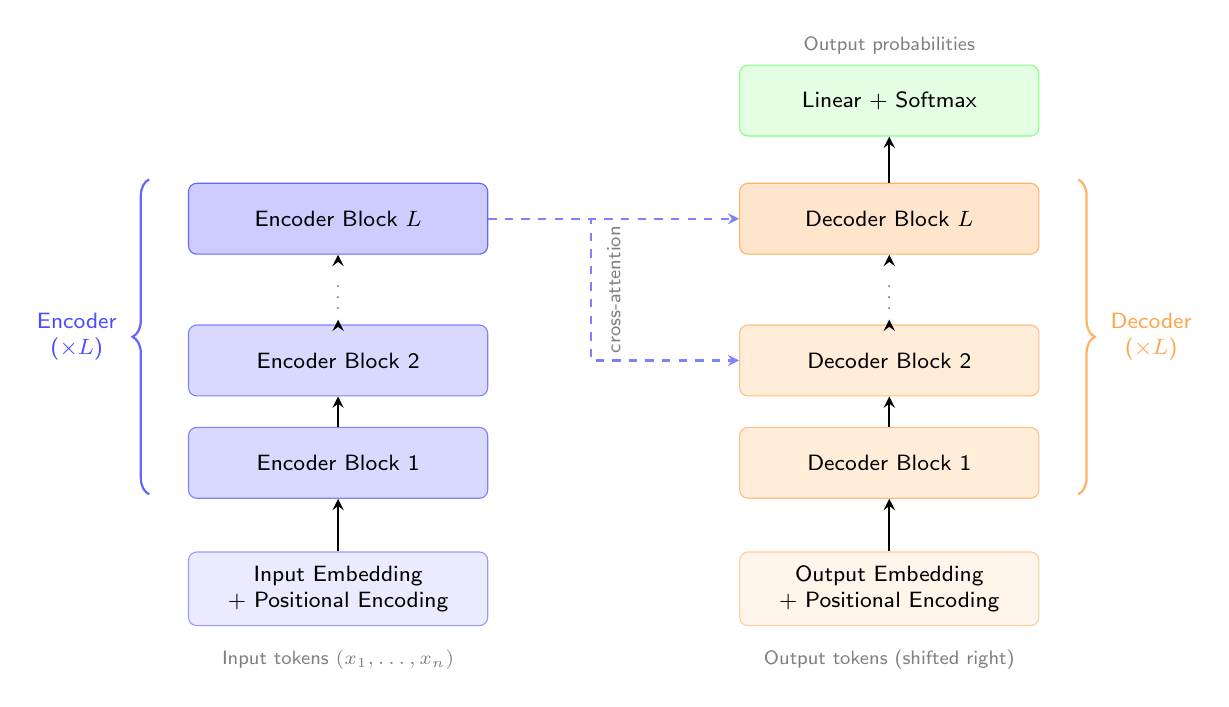
\begin{tikzpicture}[
    block/.style={draw, rounded corners=3pt, minimum width=3.8cm,
                  minimum height=0.9cm, align=center,
                  font=\footnotesize\sffamily, inner sep=5pt},
    arw/.style={->, >=stealth, thick},
    annot/.style={font=\scriptsize\sffamily, text=gray},
]
% --- Encoder Stack ---
\node[block, fill=blue!8, draw=blue!40] (emb_enc) at (0, 0)
    {Input Embedding \\ + Positional Encoding};
\node[block, fill=blue!15, draw=blue!50] (enc1) at (0, 1.6)
    {Encoder Block 1};
\node[block, fill=blue!15, draw=blue!50] (enc2) at (0, 2.9)
    {Encoder Block 2};
\node[annot] (dots_enc) at (0, 3.8) {$\vdots$};
\node[block, fill=blue!20, draw=blue!60] (encL) at (0, 4.7)
    {Encoder Block $L$};

% Encoder brace
\draw[decorate, decoration={brace, amplitude=6pt},
      thick, blue!60]
    (-2.4, 1.2) -- (-2.4, 5.2)
    node[midway, left=8pt, font=\footnotesize\sffamily,
         text=blue!70, align=center] {Encoder\\($\times L$)};

% --- Decoder Stack ---
\node[block, fill=orange!8, draw=orange!40] (emb_dec) at (7, 0)
    {Output Embedding \\ + Positional Encoding};
\node[block, fill=orange!15, draw=orange!50] (dec1) at (7, 1.6)
    {Decoder Block 1};
\node[block, fill=orange!15, draw=orange!50] (dec2) at (7, 2.9)
    {Decoder Block 2};
\node[annot] (dots_dec) at (7, 3.8) {$\vdots$};
\node[block, fill=orange!20, draw=orange!60] (decL) at (7, 4.7)
    {Decoder Block $L$};
\node[block, fill=green!10, draw=green!50] (linear) at (7, 6.2)
    {Linear + Softmax};

% Decoder brace
\draw[decorate, decoration={brace, amplitude=6pt, mirror},
      thick, orange!60]
    (9.4, 1.2) -- (9.4, 5.2)
    node[midway, right=8pt, font=\footnotesize\sffamily,
         text=orange!70, align=center] {Decoder\\($\times L$)};

% --- Main flow arrows ---
\draw[arw] (emb_enc) -- (enc1);
\draw[arw] (enc1) -- (enc2);
\draw[arw] (enc2) -- (dots_enc);
\draw[arw] (dots_enc) -- (encL);

\draw[arw] (emb_dec) -- (dec1);
\draw[arw] (dec1) -- (dec2);
\draw[arw] (dec2) -- (dots_dec);
\draw[arw] (dots_dec) -- (decL);
\draw[arw] (decL) -- (linear);

% --- Cross-attention arrows ---
\draw[arw, dashed, blue!50]
    (encL.east) -- ++(1.3, 0) |- (dec2.west);
\draw[arw, dashed, blue!50]
    (encL.east) -- ++(1.3, 0) |- (decL.west);
\node[annot, rotate=90] at (3.5, 3.8) {cross-attention};

% --- Labels (absolute positions, not relative) ---
\node[annot] at (0, -0.9) {Input tokens $(x_1, \ldots, x_n)$};
\node[annot] at (7, -0.9) {Output tokens (shifted right)};
\node[annot] at (7, 6.9) {Output probabilities};
\end{tikzpicture}%
}% end resizebox
\caption{High-level Transformer architecture. The encoder (left)
processes the input sequence through $L$ identical blocks. The decoder
(right) generates outputs auto-regressively, attending to both its own
previous tokens and the encoder's representations via cross-attention
(dashed arrows). This work focuses exclusively on the encoder.}
\label{fig:transformer_arch}
\end{figure}

In this work, we focus exclusively on the \textbf{encoder}, as our
experiments employ encoder-style self-attention for classification tasks.
The encoder consists of $L$ identical blocks stacked sequentially, where
the output of block $\ell$ serves as the input to block $\ell + 1$.

\subsubsection{Input Representation}

The encoder receives a sequence of $n$ discrete tokens, each mapped to
a $d$-dimensional continuous vector via a learned embedding matrix
$W_{\text{emb}} \in \mathbb{R}^{|V| \times d}$, where $|V|$ is the
vocabulary size. Since the attention mechanism is permutation-equivariant
(it treats all positions symmetrically), \textbf{positional encodings}
are added to inject information about token ordering:
\begin{equation}
    X^{(0)} = \text{Embed}(x_1, \ldots, x_n) + \text{PE}(1, \ldots, n)
    \;\in\; \mathbb{R}^{n \times d},
    \label{eq:input_repr}
\end{equation}
where the positional encoding $\text{PE}$ uses sinusoidal functions at
different frequencies:
\begin{align}
    \text{PE}(pos, 2i) &= \sin\!\left(\frac{pos}{10000^{2i/d}}\right), \label{eq:pe_sin} \\
    \text{PE}(pos, 2i+1) &= \cos\!\left(\frac{pos}{10000^{2i/d}}\right). \label{eq:pe_cos}
\end{align}
The exponentially decreasing frequencies across dimensions allow the
model to learn to attend to both local and global positional
relationships. Alternative approaches use learned positional embeddings,
rotary embeddings (RoPE), or ALiBi biases; we employ the original
sinusoidal scheme for consistency with the foundational architecture.

\subsubsection{Encoder Block Structure}

Each encoder block is composed of two sublayers, each wrapped with a
\textbf{residual connection}~\cite{he2016residual} and
\textbf{layer normalization}~\cite{ba2016layernorm}
(Figure~\ref{fig:encoder_block}):

\begin{figure}[H]
\centering
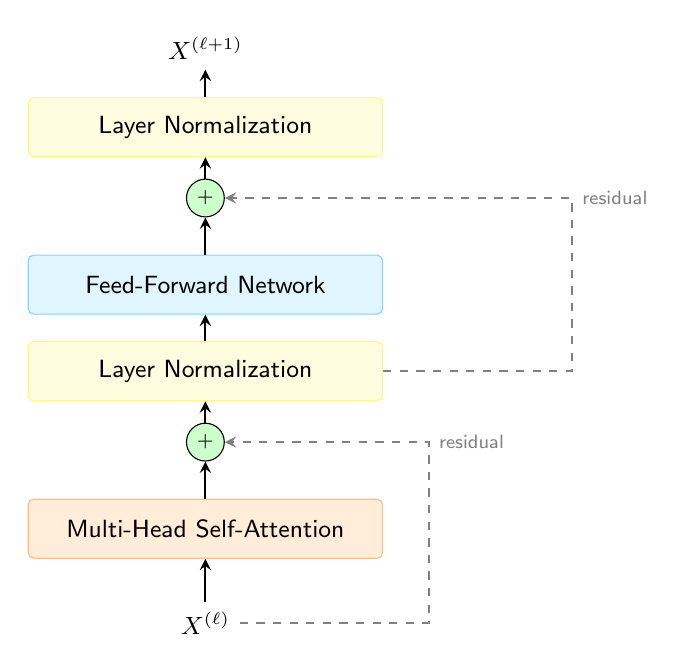
\begin{tikzpicture}[
    block/.style={draw, rounded corners=2pt, minimum width=4.5cm,
                  minimum height=0.75cm, align=center, font=\small\sffamily},
    op/.style={draw, circle, inner sep=2pt, font=\scriptsize\bfseries},
    arrow/.style={->, >=stealth, thick},
    skip/.style={->, >=stealth, thick, dashed, gray},
]
% --- Input ---
\node[font=\small\sffamily] (input) at (0, -0.5) {$X^{(\ell)}$};

% --- Multi-Head Attention ---
\node[block, fill=orange!15, draw=orange!50] (mha) at (0, 0.7)
    {Multi-Head Self-Attention};

% --- Add & Norm 1 ---
\node[op, fill=green!20] (add1) at (0, 1.8) {$+$};
\node[block, fill=yellow!12, draw=yellow!50] (ln1) at (0, 2.7)
    {Layer Normalization};

% --- FFN ---
\node[block, fill=cyan!12, draw=cyan!50] (ffn) at (0, 3.8)
    {Feed-Forward Network};

% --- Add & Norm 2 ---
\node[op, fill=green!20] (add2) at (0, 4.9) {$+$};
\node[block, fill=yellow!12, draw=yellow!50] (ln2) at (0, 5.8)
    {Layer Normalization};

% --- Output ---
\node[font=\small\sffamily] (output) at (0, 6.8) {$X^{(\ell+1)}$};

% --- Main flow ---
\draw[arrow] (input) -- (mha);
\draw[arrow] (mha) -- (add1);
\draw[arrow] (add1) -- (ln1);
\draw[arrow] (ln1) -- (ffn);
\draw[arrow] (ffn) -- (add2);
\draw[arrow] (add2) -- (ln2);
\draw[arrow] (ln2) -- (output);

% --- Residual connections ---
\draw[skip] (input.east) -- ++(2.4, 0) |- (add1.east)
    node[midway, right, font=\scriptsize\sffamily, text=gray] {residual};
\draw[skip] (ln1.east) -- ++(2.4, 0) |- (add2.east)
    node[midway, right, font=\scriptsize\sffamily, text=gray] {residual};
\end{tikzpicture}
\caption{Internal structure of a single Transformer encoder block
(Post-LN configuration). The input $X^{(\ell)}$ passes through
multi-head self-attention, is added back via a residual connection
($+$), and normalized. The result then passes through a feed-forward
network with a second residual connection and normalization to produce
$X^{(\ell+1)}$.}
\label{fig:encoder_block}
\end{figure}

Formally, the computation within encoder block $\ell$ is:
\begin{align}
    Z^{(\ell)} &= \text{LayerNorm}\!\left(X^{(\ell)}
        + \text{MHA}\!\left(X^{(\ell)}\right)\right),
        \label{eq:block_attn_full} \\
    X^{(\ell+1)} &= \text{LayerNorm}\!\left(Z^{(\ell)}
        + \text{FFN}\!\left(Z^{(\ell)}\right)\right),
        \label{eq:block_ffn_full}
\end{align}
where $\ell = 1, \ldots, L$ indexes the encoder layer, and MHA denotes
multi-head attention (detailed in Section~4.3).

\subsubsection{Position-Wise Feed-Forward Network}

The feed-forward sublayer applies an identical two-layer MLP to each
token position independently:
\begin{equation}
    \text{FFN}(z) = W_2\, \phi(W_1\, z + b_1) + b_2,
    \label{eq:ffn}
\end{equation}
where $W_1 \in \mathbb{R}^{d \times d_{\text{ff}}}$,
$W_2 \in \mathbb{R}^{d_{\text{ff}} \times d}$, and $\phi$ is a
nonlinear activation function. The original Transformer uses ReLU;
modern variants employ GELU or SwiGLU. The inner dimension
$d_{\text{ff}}$ is typically set to $4d$, providing a
\textit{bottleneck expansion} that allows the network to learn
richer per-token transformations before projecting back to
$d$~dimensions.

From a signal propagation perspective, the FFN sublayer can either
preserve or distort the singular value spectrum of the representation.
If the weights $W_1$ and $W_2$ are initialized such that
$\|W_2 W_1\|_2 \approx 1$, the FFN approximately preserves the
signal norm. However, if the gain exceeds unity, the FFN can amplify
activations and contribute to exploding gradients (see Section~4.5).

\subsubsection{Complete Encoder Data Flow}

The full data flow through the Transformer encoder can be visualized as
a pipeline (Figure~\ref{fig:encoder_flow}):

\begin{figure}[H]
\centering
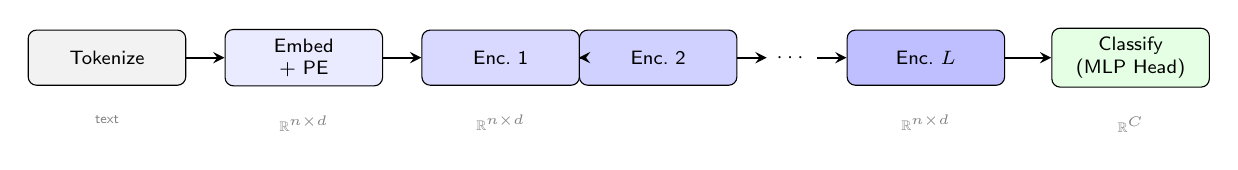
\begin{tikzpicture}[
    stage/.style={draw, rounded corners=3pt, minimum height=0.7cm,
                  align=center, font=\scriptsize\sffamily, minimum width=2.0cm},
    arrow/.style={->, >=stealth, thick},
]
\node[stage, fill=gray!10] (tok) at (0, 0) {Tokenize};
\node[stage, fill=blue!8] (emb) at (2.5, 0) {Embed\\$+$ PE};
\node[stage, fill=blue!15] (e1) at (5.0, 0) {Enc.~1};
\node[stage, fill=blue!18] (e2) at (7.0, 0) {Enc.~2};
\node[font=\scriptsize\sffamily] (dots) at (8.7, 0) {$\cdots$};
\node[stage, fill=blue!25] (eL) at (10.4, 0) {Enc.~$L$};
\node[stage, fill=green!10] (cls) at (13.0, 0) {Classify\\(MLP Head)};

\draw[arrow] (tok) -- (emb);
\draw[arrow] (emb) -- (e1);
\draw[arrow] (e1) -- (e2);
\draw[arrow] (e2) -- (dots);
\draw[arrow] (dots) -- (eL);
\draw[arrow] (eL) -- (cls);

% Dimension annotations
\node[below=0.25cm, font=\tiny\sffamily, text=gray] at (tok.south) {text};
\node[below=0.25cm, font=\tiny\sffamily, text=gray] at (emb.south)
    {$\mathbb{R}^{n \times d}$};
\node[below=0.25cm, font=\tiny\sffamily, text=gray] at (e1.south)
    {$\mathbb{R}^{n \times d}$};
\node[below=0.25cm, font=\tiny\sffamily, text=gray] at (eL.south)
    {$\mathbb{R}^{n \times d}$};
\node[below=0.25cm, font=\tiny\sffamily, text=gray] at (cls.south)
    {$\mathbb{R}^{C}$};
\end{tikzpicture}
\caption{Data flow through the Transformer encoder. The representation
dimensionality $\mathbb{R}^{n \times d}$ is preserved across all
$L$ encoder blocks. The classification head (used in our experiments)
pools the sequence and projects to $C$ classes.}
\label{fig:encoder_flow}
\end{figure}

\noindent
The key observation is that the representation dimensionality
$\mathbb{R}^{n \times d}$ is \textit{preserved} across all $L$ encoder
blocks. Each block is a residual mapping that transforms the
representation without changing its shape. This uniformity makes it
particularly straightforward to track how the \textit{quality} of the
representation---as measured by stable rank---evolves across depth,
since the matrices at each layer have identical dimensions.

\subsubsection{Summary of Architectural Components}

Table~\ref{tab:arch_components} summarizes the key components and their
roles in signal propagation.

\begin{table}[H]
\centering
\caption{Transformer encoder components and their roles in signal
propagation. Components marked with $\dagger$ are removed in our
vanilla attention baseline to isolate the raw attention mechanism.}
\label{tab:arch_components}
\begin{tabular}{@{}llc@{}}
\toprule
\textbf{Component} & \textbf{Role in Signal Propagation} & \textbf{In Vanilla?} \\
\midrule
Token Embedding     & Maps discrete tokens to $\mathbb{R}^d$ & \checkmark \\
Positional Encoding & Injects position information & \checkmark \\
Multi-Head Attention & Computes inter-token dependencies & \checkmark \\
Feed-Forward Network & Per-token nonlinear transformation & \checkmark \\
Residual Connection$^\dagger$ & Preserves signal floor via identity bypass & $\times$ \\
Layer Normalization$^\dagger$ & Stabilizes scale, counteracts collapse & $\times$ \\
Classification Head  & Pools and projects to class logits & \checkmark \\
\bottomrule
\end{tabular}
\end{table}

\subsection{Scaled Dot-Product Attention}

The atomic operation within the Transformer is \textbf{scaled dot-product
attention}. Given query, key, and value matrices $Q, K \in
\mathbb{R}^{n \times d_k}$ and $V \in \mathbb{R}^{n \times d_v}$,
the attention output is:
\begin{equation}
    \text{Attention}(Q, K, V) = \underbrace{\text{softmax}\!\left(\frac{QK^\top}{\sqrt{d_k}}\right)}_{A \;\in\; \mathbb{R}^{n \times n}} V,
    \label{eq:sdpa_detail}
\end{equation}
where the softmax is applied row-wise. We denote the attention matrix as
$A = \text{softmax}(S / \sqrt{d_k})$, where $S = QK^\top \in
\mathbb{R}^{n \times n}$ is the raw score matrix.

\paragraph{Properties of the attention matrix.}
The softmax operation endows $A$ with two important properties:
\begin{enumerate}[label=(\alph*)]
    \item \textbf{Non-negativity:} $A_{ij} \geq 0$ for all $i, j$.
    \item \textbf{Row-stochasticity:} $\sum_{j=1}^{n} A_{ij} = 1$
          for all $i$.
\end{enumerate}
Thus $A$ is a \textit{right stochastic matrix} (or Markov matrix).
This structure has profound spectral consequences: by the
Perron-Frobenius theorem, the largest singular value of $A$ satisfies
$\sigma_1(A) = 1$, and the corresponding right singular vector is
proportional to $\mathbf{1}_n$.

\paragraph{Geometric interpretation.}
The attention operation $\hat{V} = AV$ computes each output token as a
convex combination of the value vectors. When $A$ is close to the
\textit{uniform} attention matrix $\mathbf{1}\mathbf{1}^\top / n$, all
output tokens converge to the same vector (the mean of the values),
destroying all token-level information. When $A$ is close to the
identity, each token retains its original value. The spectral structure
of $A$ determines where on this continuum the output falls.

\subsection{Multi-Head Attention}

Multi-head attention decomposes the attention computation into $h$
parallel \textit{heads}, each operating on a learned linear projection
of the input:
\begin{equation}
    \text{MultiHead}(X) = \text{Concat}\!\left(\text{head}_1, \ldots, \text{head}_h\right) W^O,
    \label{eq:mha_detail}
\end{equation}
where
\begin{equation}
    \text{head}_i = \text{Attention}\!\left(X W_i^Q,\; X W_i^K,\; X W_i^V\right),
    \label{eq:head_i}
\end{equation}
with projection matrices $W_i^Q, W_i^K \in \mathbb{R}^{d \times d_k}$,
$W_i^V \in \mathbb{R}^{d \times d_v}$, and output projection
$W^O \in \mathbb{R}^{hd_v \times d}$. Typically $d_k = d_v = d / h$.

Each head produces its own attention matrix $A_i \in
\mathbb{R}^{n \times n}$. The spectral properties of these individual
attention matrices---and particularly their stable rank---are the primary
objects of study in this work. Even if the output projection $W^O$ mixes
information across heads, the rank collapse occurring within any single
head's attention matrix still constrains the representational capacity of
that head.

\subsection{Residual Connections and Layer Normalization}

\paragraph{Residual connections.}
The residual connection~\cite{he2016residual} adds the sublayer input
directly to its output:
\begin{equation}
    y = x + f(x),
    \label{eq:residual}
\end{equation}
where $f$ represents the sublayer function (attention or FFN). Consider
the effect on singular values. If $f(x) = Mx$ for a linear map $M$,
then $y = (I + M)x$. The singular values of $(I + M)$ are
$1 + \sigma_i(M) \cos\theta_i$, where $\theta_i$ are the principal
angles between the singular subspaces of $I$ and $M$. Crucially, even if
$\sigma_i(M) \to 0$ (complete signal loss in the sublayer), the
identity component ensures $\sigma_i(I + M) \geq 1 - |\sigma_i(M)|$,
preventing total rank collapse.

\paragraph{Layer normalization.}
Layer normalization~\cite{ba2016layernorm} normalizes each token's
representation across the feature dimension:
\begin{equation}
    \text{LayerNorm}(x) = \gamma \odot \frac{x - \mu}{\sqrt{\sigma^2 + \epsilon}} + \beta,
    \label{eq:layernorm}
\end{equation}
where $\mu = \frac{1}{d}\sum_{i=1}^d x_i$ and $\sigma^2 =
\frac{1}{d}\sum_{i=1}^d (x_i - \mu)^2$ are the per-token mean and
variance, and $\gamma, \beta \in \mathbb{R}^d$ are learnable scale and
shift parameters.

From a spectral perspective, layer normalization performs two operations
relevant to signal propagation:
\begin{enumerate}[label=(\roman*)]
    \item \textbf{Centering} ($x \mapsto x - \mu$): Projects out the
          component along $\mathbf{1}_d$, which is precisely the
          direction associated with rank collapse in the attention
          output.
    \item \textbf{Rescaling} ($x \mapsto x / \sigma$): Normalizes the
          magnitude of the representation, preventing the exponential
          growth or decay that leads to exploding or vanishing
          activations.
\end{enumerate}
The combination of residual connections and layer normalization thus
provides a two-pronged defense against rank collapse: the residual
preserves a minimum signal floor, while the normalization prevents
scale drift and partially counteracts the directional collapse induced
by the attention matrix.

\subsection{Vanishing and Exploding Gradients in Transformers}

Consider a stack of $L$ vanilla attention layers (without residuals or
normalization), where the forward pass is:
\begin{equation}
    X^{(\ell+1)} = A^{(\ell)} X^{(\ell)}, \qquad \ell = 1, \ldots, L.
    \label{eq:vanilla_forward}
\end{equation}
The end-to-end mapping from input to output is:
\begin{equation}
    X^{(L+1)} = \left(\prod_{\ell=1}^{L} A^{(\ell)}\right) X^{(1)}.
    \label{eq:product}
\end{equation}
The Jacobian of this mapping with respect to the input is the product
of attention matrices $\prod_{\ell} A^{(\ell)}$.

\paragraph{Singular value analysis.}
Let $\sigma_1^{(\ell)} \geq \sigma_2^{(\ell)} \geq \cdots \geq
\sigma_n^{(\ell)}$ denote the singular values of $A^{(\ell)}$. For the
product of $L$ layers, the singular values satisfy (by submultiplicativity):
\begin{equation}
    \sigma_i\!\left(\prod_{\ell=1}^{L} A^{(\ell)}\right) \leq
    \prod_{\ell=1}^{L} \sigma_i\!\left(A^{(\ell)}\right).
    \label{eq:sv_bound}
\end{equation}
Since each $A^{(\ell)}$ is row-stochastic, $\sigma_1^{(\ell)} = 1$. If
the spectral gap is such that $\sigma_2^{(\ell)} = \rho < 1$ for all
$\ell$, then:
\begin{equation}
    \sigma_2\!\left(\prod_{\ell=1}^{L} A^{(\ell)}\right)
    \leq \rho^L \xrightarrow{L \to \infty} 0.
    \label{eq:vanishing}
\end{equation}
This is the mechanism of \textbf{vanishing gradients}: all singular
values except $\sigma_1$ decay exponentially with depth, causing the
gradient information along all but one direction to be lost.

\paragraph{Exploding gradients.}
In the presence of the feed-forward sublayer and learned projections,
the effective Jacobian is no longer purely a product of stochastic
matrices. If the FFN amplifies activations (e.g., through a gain greater
than unity), the singular values of the per-layer Jacobian can exceed 1,
leading to exponential growth:
\begin{equation}
    \sigma_i\!\left(J^{(1:L)}\right) \sim \gamma^L, \quad \gamma > 1
    \implies \text{exploding gradients}.
    \label{eq:exploding}
\end{equation}

\paragraph{The critical regime.}
Healthy signal propagation requires all singular values of the per-layer
Jacobian to be close to unity---the so-called \textit{edge of chaos} or
\textit{dynamical isometry} condition:
\begin{equation}
    \sigma_i(J^{(\ell)}) \approx 1, \quad \forall\, i, \ell.
    \label{eq:isometry}
\end{equation}
Achieving this condition without explicit interventions (residuals, normalization) is precisely the challenge that motivates investigating alternative attention mechanisms.

\subsection{Differential Attention Mechanism}

The differential attention mechanism~\cite{diff_transformer} modifies the
standard attention computation by splitting the query and key projections
into two halves and computing the attention output as a difference of two
attention maps. Formally, for an input $X \in \mathbb{R}^{n \times d}$:

\paragraph{Step 1: Dual projections.}
\begin{equation}
    Q_1 = X W_1^Q, \quad Q_2 = X W_2^Q, \quad
    K_1 = X W_1^K, \quad K_2 = X W_2^K, \quad
    V = X W^V,
    \label{eq:diff_proj}
\end{equation}
where $W_1^Q, W_2^Q, W_1^K, W_2^K \in \mathbb{R}^{d \times d_k}$ and
$W^V \in \mathbb{R}^{d \times d_v}$.

\paragraph{Step 2: Dual attention maps.}
\begin{align}
    A_1 &= \text{softmax}\!\left(\frac{Q_1 K_1^\top}{\sqrt{d_k}}\right)
    \in \mathbb{R}^{n \times n}, \label{eq:A1} \\
    A_2 &= \text{softmax}\!\left(\frac{Q_2 K_2^\top}{\sqrt{d_k}}\right)
    \in \mathbb{R}^{n \times n}. \label{eq:A2}
\end{align}
Both $A_1$ and $A_2$ are independently row-stochastic.

\paragraph{Step 3: Differential output.}
\begin{equation}
    \text{DiffAttn}(X) = \left(A_1 - \lambda\, A_2\right) V,
    \label{eq:diff_output}
\end{equation}
where $\lambda \in \mathbb{R}$ is a learnable scalar initialized to a
small value (typically $\lambda_{\text{init}} \approx 0.05$).

\paragraph{Spectral analysis of differential attention.}
The differential attention matrix $A_{\text{diff}} = A_1 - \lambda A_2$
is \textit{not} row-stochastic (rows sum to $1 - \lambda$, and entries
can be negative). Its spectral properties differ markedly from a single
softmax attention matrix:
\begin{itemize}[leftmargin=1.5em]
    \item The leading singular value is reduced from $\sigma_1 = 1$ to
          approximately $\sigma_1 \approx 1 - \lambda$, since the
          uniform component of $A_1$ and $A_2$ (which contributes to
          $\sigma_1$) is partially cancelled.
    \item The \textbf{spectral gap} $(\sigma_1 - \sigma_2)$ is
          consequently \textit{narrowed}, as the common-mode uniform
          component---which is the primary source of the gap---is
          suppressed by the subtraction.
    \item The \textbf{stable rank} of $A_{\text{diff}}$ is expected to
          be higher than that of $A_1$ or $A_2$ individually, reflecting
          a more distributed singular value spectrum.
\end{itemize}

\subsection{Mind the Gap Attention Mechanism}

The ``Mind the Gap'' framework~\cite{mind_the_gap} diagnoses the spectral
gap as the root cause of rank collapse and proposes a direct spectral
correction to the attention matrix. We formalize this correction as a
self-contained attention mechanism.

\paragraph{Step 1: Standard attention matrix.}
Compute the standard softmax attention matrix:
\begin{equation}
    A = \text{softmax}\!\left(\frac{QK^\top}{\sqrt{d_k}}\right)
    \in \mathbb{R}^{n \times n}.
    \label{eq:mtg_standard}
\end{equation}

\paragraph{Step 2: Singular value decomposition.}
Compute the SVD of the attention matrix:
\begin{equation}
    A = U \Sigma V^\top = \sum_{i=1}^{n} \sigma_i\, \mathbf{u}_i \mathbf{v}_i^\top,
    \label{eq:mtg_svd}
\end{equation}
where $\sigma_1 \geq \sigma_2 \geq \cdots \geq \sigma_n \geq 0$.

\paragraph{Step 3: Spectral gap identification.}
The spectral gap is defined as:
\begin{equation}
    \Delta = \sigma_1 - \sigma_2.
    \label{eq:spectral_gap}
\end{equation}
When $\Delta$ is large, the attention matrix is dominated by its
rank-one component $\sigma_1 \mathbf{u}_1 \mathbf{v}_1^\top$, which
maps all input tokens toward the same direction.

\paragraph{Step 4: Spectral gap correction.}
The corrected attention matrix is obtained by dampening or removing the
outlier singular value:
\begin{equation}
    A_{\text{corrected}} = U\, \tilde{\Sigma}\, V^\top, \quad
    \text{where} \quad
    \tilde{\sigma}_i =
    \begin{cases}
        \sigma_2 & \text{if } i = 1 \text{ (clamp to bulk)}, \\
        \sigma_i & \text{otherwise}.
    \end{cases}
    \label{eq:mtg_correction}
\end{equation}
An alternative formulation projects out the rank-one component entirely:
\begin{equation}
    A_{\text{corrected}} = A - \sigma_1\, \mathbf{u}_1 \mathbf{v}_1^\top
    + \sigma_2\, \mathbf{u}_1 \mathbf{v}_1^\top
    = A - \Delta\, \mathbf{u}_1 \mathbf{v}_1^\top.
    \label{eq:mtg_projection}
\end{equation}

\paragraph{Step 5: Corrected output.}
\begin{equation}
    \text{MtGAttn}(X) = A_{\text{corrected}}\, V.
    \label{eq:mtg_output}
\end{equation}

\paragraph{Spectral properties of the corrected matrix.}
By construction, the corrected attention matrix satisfies:
\begin{enumerate}[label=(\roman*)]
    \item $\sigma_1(A_{\text{corrected}}) = \sigma_2(A)$, eliminating
          the spectral gap.
    \item The stable rank increases:
    \begin{equation}
        r(A_{\text{corrected}}) =
        \frac{\|A_{\text{corrected}}\|_F^2}{\|A_{\text{corrected}}\|_2^2}
        = \frac{\sum_{i=2}^{n} \sigma_i^2 + \sigma_2^2}
               {\sigma_2^2}
        > \frac{\sum_{i=1}^{n} \sigma_i^2}{\sigma_1^2}
        = r(A),
        \label{eq:mtg_stable_rank}
    \end{equation}
    since the denominator decreases ($\sigma_2^2 < \sigma_1^2$) while
    the numerator remains comparable.
    \item The Jacobian of the corrected layer has a flatter singular
          value distribution, promoting dynamical isometry and
          healthier gradient flow.
\end{enumerate}

\paragraph{Computational cost.}
The SVD in Step 2 incurs $\mathcal{O}(n^3)$ cost, which can be
prohibitive for long sequences. In practice, a truncated SVD or
power-iteration estimate of $\sigma_1$ and $\mathbf{u}_1$ suffices,
reducing the overhead to $\mathcal{O}(n^2 k)$ for $k$ iterations.

\subsection{Rank Collapse in Transformers}

We now formalize the two modes of rank collapse identified in the
literature and connect them to the attention matrix's spectral structure.

\paragraph{Rank collapse in depth.}
Consider the output after $L$ layers of vanilla attention
(Eq.~\ref{eq:product}). The effective operator is
$\mathcal{A} = \prod_{\ell=1}^{L} A^{(\ell)}$. If each $A^{(\ell)}$
has a spectral gap $\Delta^{(\ell)}$ with second singular value
$\rho^{(\ell)} < 1$, then the product converges to a rank-one matrix:
\begin{equation}
    \lim_{L \to \infty} \prod_{\ell=1}^{L} A^{(\ell)}
    = \mathbf{u}\, \boldsymbol{\pi}^\top,
    \label{eq:rank_one_limit}
\end{equation}
where $\boldsymbol{\pi}$ is the stationary distribution of the
Markov chain defined by the product of stochastic matrices. In this
limit, all input tokens are mapped to the \textit{same} output vector,
destroying all discriminative information. The rate of convergence is
governed by $\max_\ell \rho^{(\ell)}$: the larger the spectral gap,
the faster the collapse.

\paragraph{Rank collapse in width.}
Even within a \textit{single} attention layer, as the context length
$n$ increases, the attention matrix $A$ becomes increasingly close to
the uniform matrix $\mathbf{1}\mathbf{1}^\top / n$. This is because the
softmax operates on $n$ logits that, at random initialization, are
approximately i.i.d.\ Gaussian; as $n$ grows, the softmax output
concentrates around the uniform distribution by a law-of-large-numbers
effect~\cite{mind_the_gap}.

Formally, at initialization with random weights, the score matrix
$S = QK^\top / \sqrt{d_k}$ has entries $S_{ij} \sim \mathcal{N}(0, 1)$.
The softmax of a row of $n$ i.i.d.\ standard Gaussians yields an
attention vector that concentrates around $(1/n, \ldots, 1/n)$ as
$n \to \infty$. The resulting attention matrix has:
\begin{equation}
    \sigma_1(A) \to 1, \quad \sigma_2(A) \to 0
    \quad \text{as } n \to \infty,
    \label{eq:width_collapse}
\end{equation}
i.e., the stable rank of $A$ converges to 1, regardless of the
embedding dimension $d$.

\paragraph{Combined effect.}
The two modes of collapse are synergistic: rank collapse in width
produces attention matrices with large spectral gaps, which then
compound across layers via rank collapse in depth. The result is that
deep, wide-context vanilla Transformers suffer doubly accelerated signal
degradation---a ``collapse amplification'' that makes training without
stabilization infeasible.

\subsection{Stable Rank as a Diagnostic Metric}

\paragraph{Definition.}
The \textbf{stable rank} of a matrix $A \in \mathbb{R}^{m \times n}$
is defined as:
\begin{equation}
    \boxed{\;
    r(A) = \frac{\|A\|_F^2}{\|A\|_2^2}
    = \frac{\sum_{i=1}^{\min(m,n)} \sigma_i^2}{\sigma_1^2}
    \;}
    \label{eq:stable_rank_def}
\end{equation}
where $\|A\|_F = \sqrt{\sum_{i} \sigma_i^2}$ is the Frobenius norm and
$\|A\|_2 = \sigma_1$ is the spectral norm (largest singular value).

\paragraph{Interpretation.}
The stable rank is a continuous, differentiable relaxation of the
algebraic rank that measures how ``spread out'' the singular values are:
\begin{itemize}[leftmargin=1.5em]
    \item \textbf{Maximum stable rank:} $r(A) = \text{rank}(A)$ when
          all nonzero singular values are equal (i.e., the matrix is a
          scaled partial isometry). This represents the healthiest
          possible signal propagation---no direction is preferred over
          any other.
    \item \textbf{Minimum stable rank:} $r(A) = 1$ when the matrix
          has exactly one nonzero singular value (rank-one matrix).
          This is the degenerate case corresponding to complete rank
          collapse.
    \item \textbf{General bound:} $1 \leq r(A) \leq \text{rank}(A)$
          always holds.
\end{itemize}

\paragraph{Stable rank of attention matrices.}
For a row-stochastic attention matrix $A$ with singular values
$1 = \sigma_1 \geq \sigma_2 \geq \cdots \geq \sigma_n \geq 0$:
\begin{equation}
    r(A) = 1 + \sum_{i=2}^{n} \sigma_i^2.
    \label{eq:sr_attention}
\end{equation}
Thus, the stable rank equals $1$ plus the sum of squared sub-leading
singular values. A small spectral gap (large $\sigma_2, \ldots,
\sigma_n$) yields a high stable rank; a large spectral gap
($\sigma_i \to 0$ for $i \geq 2$) drives the stable rank toward 1.

\paragraph{Stable rank as a predictor of trainability.}
We hypothesize---and empirically validate---that the stable rank of
attention matrices at initialization and during training serves as a
reliable predictor of:
\begin{enumerate}[label=(\roman*)]
    \item \textbf{Signal preservation:} Higher stable rank implies more
          directions of information flow, reducing the risk of losing
          discriminative features.
    \item \textbf{Gradient health:} Higher stable rank in the Jacobian
          correlates with more directions along which gradients can
          propagate, mitigating vanishing gradients.
    \item \textbf{Final performance:} Models whose attention layers
          maintain high stable rank throughout training achieve
          lower validation error and higher accuracy.
\end{enumerate}

\paragraph{Comparison with alternative metrics.}
Table~\ref{tab:metrics_comparison} summarizes the key diagnostic metrics
and their trade-offs.

\begin{table}[H]
\centering
\caption{Comparison of spectral diagnostic metrics for attention matrices.}
\label{tab:metrics_comparison}
\begin{tabular}{@{}lccc@{}}
\toprule
\textbf{Metric} & \textbf{Formula} & \textbf{Range} & \textbf{Computational Cost} \\
\midrule
Algebraic Rank  & $\#\{\sigma_i > 0\}$ & $[1, n]$ & $\mathcal{O}(n^3)$ \\
Condition Number & $\sigma_1 / \sigma_n$ & $[1, \infty)$ & $\mathcal{O}(n^3)$ \\
Effective Rank  & $\exp\!\left(-\sum p_i \log p_i\right)$ & $[1, n]$ & $\mathcal{O}(n^3)$ \\
\textbf{Stable Rank}  & $\|A\|_F^2 / \|A\|_2^2$ & $[1, n]$ & $\mathcal{O}(n^2)$\textsuperscript{*} \\
\bottomrule
\end{tabular}
\par\smallskip
\raggedright\small\textsuperscript{*}Requires only $\|A\|_F^2$ (trivial) and $\sigma_1$ (via power iteration in $\mathcal{O}(n^2 k)$).
\end{table}

Stable rank offers the best balance of interpretability, robustness (it
is insensitive to near-zero singular values, unlike the condition number),
and computational efficiency (it does not require the full SVD, unlike
effective rank).

% -----------------------------------------------------------------------------
% 5. SYSTEM DESIGN & IMPLEMENTATION
% -----------------------------------------------------------------------------
\section{System Design and Implementation}

This section describes the concrete system built to conduct the
experiments reported in this work. We detail the hybrid
CNN--Transformer architecture used for image classification, the four
attention variants implemented, the datasets employed, the training
pipeline with explicit tensor-dimension tracking for a $32 \times 32$
input image, the software stack, and the interactive web application
(\textit{Synthetic Observer}) that provides real-time visualization of
training dynamics.

\subsection{Overall Architecture}

Unlike the standard Vision Transformer (ViT), which splits an image into
non-overlapping patches and projects each patch linearly to form a token
sequence, our architecture employs a \textbf{hybrid CNN--Transformer}
design. A convolutional front-end extracts local spatial features and
reduces spatial dimensions, producing a compact feature vector that is
then processed by a stack of self-attention blocks.

The rationale for this hybrid approach is twofold:
\begin{enumerate}[label=(\roman*)]
    \item \textbf{Focus on attention:} By delegating low-level feature
          extraction to convolutions, we isolate the attention
          mechanism's contribution to signal propagation. Any observed
          rank collapse or gradient pathology can be attributed to the
          attention layers rather than the feature extractor.
    \item \textbf{Computational efficiency:} Operating attention on a
          single 128-dimensional token (rather than $16 \times 16 = 256$
          patch tokens) allows rapid experimentation across many
          hyperparameter configurations.
\end{enumerate}

The overall pipeline is illustrated in Figure~\ref{fig:hybrid_arch}.

\begin{figure}[H]
\centering
\resizebox{0.95\textwidth}{!}{%
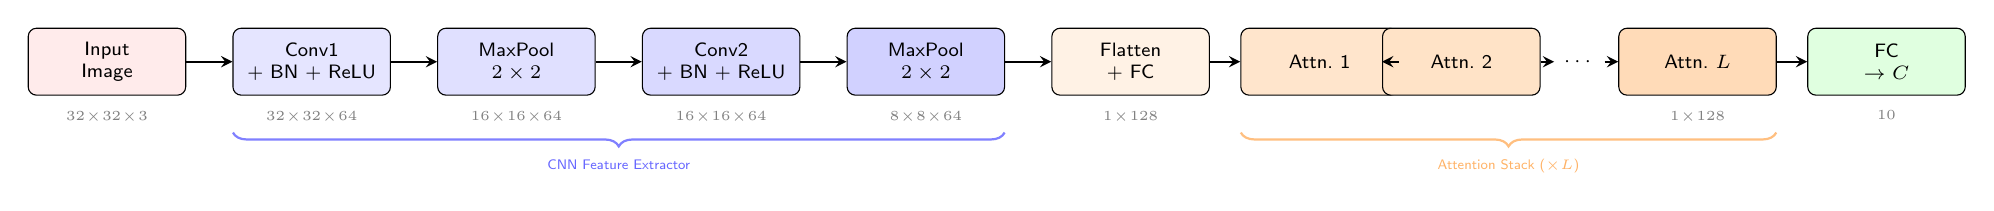
\begin{tikzpicture}[
    stage/.style={draw, rounded corners=3pt, minimum height=0.85cm,
                  align=center, font=\scriptsize\sffamily,
                  minimum width=2.0cm, inner sep=4pt},
    arw/.style={->, >=stealth, thick},
    dim/.style={font=\tiny\sffamily, text=gray},
]
\node[stage, fill=red!8] (img) at (0, 0) {Input\\Image};
\node[stage, fill=blue!10] (c1) at (2.6, 0) {Conv1\\+ BN + ReLU};
\node[stage, fill=blue!12] (p1) at (5.2, 0) {MaxPool\\$2\times 2$};
\node[stage, fill=blue!15] (c2) at (7.8, 0) {Conv2\\+ BN + ReLU};
\node[stage, fill=blue!18] (p2) at (10.4, 0) {MaxPool\\$2\times 2$};
\node[stage, fill=orange!10] (flat) at (13.0, 0) {Flatten\\+ FC};
\node[stage, fill=orange!20] (a1) at (15.4, 0) {Attn.~1};
\node[stage, fill=orange!22] (a2) at (17.2, 0) {Attn.~2};
\node[font=\scriptsize\sffamily] (dots) at (18.7, 0) {$\cdots$};
\node[stage, fill=orange!28] (aL) at (20.2, 0) {Attn.~$L$};
\node[stage, fill=green!12] (cls) at (22.6, 0) {FC\\$\to C$};

\draw[arw] (img) -- (c1);
\draw[arw] (c1) -- (p1);
\draw[arw] (p1) -- (c2);
\draw[arw] (c2) -- (p2);
\draw[arw] (p2) -- (flat);
\draw[arw] (flat) -- (a1);
\draw[arw] (a1) -- (a2);
\draw[arw] (a2) -- (dots);
\draw[arw] (dots) -- (aL);
\draw[arw] (aL) -- (cls);

% Dimension labels
\node[dim, below=2pt] at (img.south) {$32\!\times\!32\!\times\!3$};
\node[dim, below=2pt] at (c1.south) {$32\!\times\!32\!\times\!64$};
\node[dim, below=2pt] at (p1.south) {$16\!\times\!16\!\times\!64$};
\node[dim, below=2pt] at (c2.south) {$16\!\times\!16\!\times\!64$};
\node[dim, below=2pt] at (p2.south) {$8\!\times\!8\!\times\!64$};
\node[dim, below=2pt] at (flat.south) {$1\!\times\!128$};
\node[dim, below=2pt] at (aL.south) {$1\!\times\!128$};
\node[dim, below=2pt] at (cls.south) {$10$};

% Grouping braces
\draw[decorate, decoration={brace, amplitude=5pt, mirror}, thick, blue!50]
    (1.6, -0.9) -- (11.4, -0.9)
    node[midway, below=6pt, font=\tiny\sffamily, text=blue!60]
    {CNN Feature Extractor};
\draw[decorate, decoration={brace, amplitude=5pt, mirror}, thick, orange!50]
    (14.4, -0.9) -- (21.2, -0.9)
    node[midway, below=6pt, font=\tiny\sffamily, text=orange!60]
    {Attention Stack ($\times L$)};
\end{tikzpicture}%
}
\caption{Hybrid CNN--Transformer architecture for $32 \times 32$ image
classification. The convolutional front-end reduces spatial dimensions
and extracts features; the attention stack processes the resulting
128-dimensional token through $L$ self-attention blocks; the linear
head produces class logits.}
\label{fig:hybrid_arch}
\end{figure}

\subsubsection{Vision Transformer (Architecture B)}

The differential and Mind the Gap attention experiments employ a
\textbf{standard Vision Transformer (ViT)} architecture, which operates
on a sequence of image patch tokens rather than a single CNN-derived
feature vector. This full-sequence design produces attention matrices
$A \in \mathbb{R}^{n \times n}$ with $n = 65$ tokens, providing
meaningful spectral structure for stable rank analysis.

The ViT tokenization process for a $32 \times 32 \times 3$ input image
proceeds as follows:
\begin{enumerate}[label=(\roman*)]
    \item \textbf{Patch extraction:} The image is divided into
          non-overlapping patches of size $P \times P = 4 \times 4$,
          yielding $(32 / 4)^2 = 64$ patches, each a flattened vector
          of dimension $P^2 \cdot C = 4^2 \cdot 3 = 48$.
    \item \textbf{Linear projection:} Each patch is projected to
          $d = 128$ dimensions via a convolutional layer
          \texttt{Conv2d}$(3 \to 128, \; 4 \times 4, \;
          \text{stride} = 4)$, producing a patch embedding matrix
          $X_{\text{patches}} \in \mathbb{R}^{64 \times 128}$.
    \item \textbf{CLS token:} A learnable classification token
          $z_{\text{cls}} \in \mathbb{R}^{1 \times 128}$ is prepended
          to the patch sequence:
          $\tilde{X} = [z_{\text{cls}};\, X_{\text{patches}}]
          \in \mathbb{R}^{65 \times 128}$.
    \item \textbf{Positional encoding:} Learnable positional embeddings
          $E_{\text{pos}} \in \mathbb{R}^{65 \times 128}$ are added
          element-wise:
          $X^{(0)} = \tilde{X} + E_{\text{pos}}$.
    \item \textbf{Transformer encoder:} The token sequence passes
          through $L = 6$ Pre-LN Transformer blocks (described below).
    \item \textbf{Classification:} A final LayerNorm is applied, the
          CLS token is extracted ($x^{(L)}_0 \in \mathbb{R}^{128}$),
          and a linear head projects it to $C = 10$ class logits.
\end{enumerate}

The complete ViT pipeline is illustrated in
Figure~\ref{fig:vit_arch}.

\begin{figure}[H]
\centering
\resizebox{0.95\textwidth}{!}{%
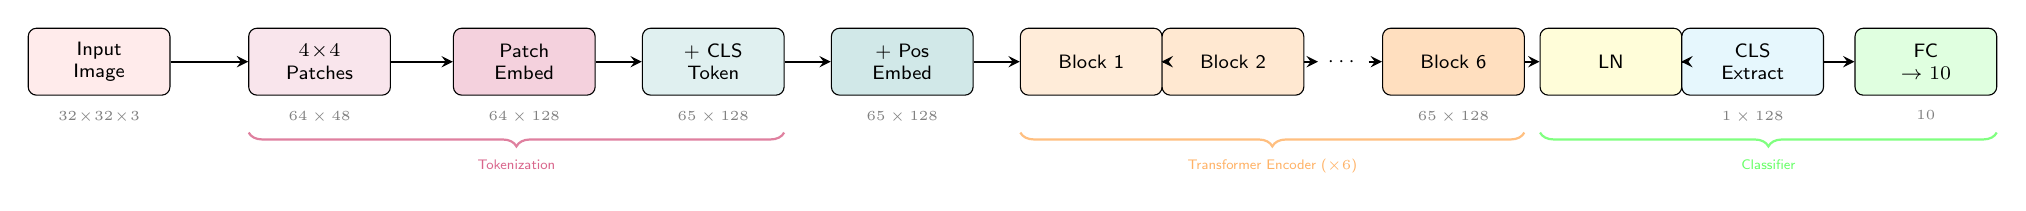
\begin{tikzpicture}[
    stage/.style={draw, rounded corners=3pt, minimum height=0.85cm,
                  align=center, font=\scriptsize\sffamily,
                  minimum width=1.8cm, inner sep=4pt},
    arw/.style={->, >=stealth, thick},
    dim/.style={font=\tiny\sffamily, text=gray},
]
% --- Nodes ---
\node[stage, fill=red!8] (img) at (0, 0) {Input\\Image};
\node[stage, fill=purple!10] (patch) at (2.8, 0)
    {$4\!\times\!4$\\Patches};
\node[stage, fill=purple!18] (proj) at (5.4, 0)
    {Patch\\Embed};
\node[stage, fill=teal!12] (cls) at (7.8, 0)
    {+ CLS\\Token};
\node[stage, fill=teal!18] (pos) at (10.2, 0)
    {+ Pos\\Embed};
\node[stage, fill=orange!15] (b1) at (12.6, 0)
    {Block 1};
\node[stage, fill=orange!18] (b2) at (14.4, 0)
    {Block 2};
\node[font=\scriptsize\sffamily] (dots) at (15.8, 0) {$\cdots$};
\node[stage, fill=orange!25] (bL) at (17.2, 0)
    {Block 6};
\node[stage, fill=yellow!15] (ln) at (19.2, 0)
    {LN};
\node[stage, fill=cyan!10] (ext) at (21.0, 0)
    {CLS\\Extract};
\node[stage, fill=green!12] (fc) at (23.2, 0)
    {FC\\$\to 10$};

% --- Arrows ---
\draw[arw] (img) -- (patch);
\draw[arw] (patch) -- (proj);
\draw[arw] (proj) -- (cls);
\draw[arw] (cls) -- (pos);
\draw[arw] (pos) -- (b1);
\draw[arw] (b1) -- (b2);
\draw[arw] (b2) -- (dots);
\draw[arw] (dots) -- (bL);
\draw[arw] (bL) -- (ln);
\draw[arw] (ln) -- (ext);
\draw[arw] (ext) -- (fc);

% --- Dimension labels ---
\node[dim, below=2pt] at (img.south) {$32\!\times\!32\!\times\!3$};
\node[dim, below=2pt] at (patch.south) {$64 \times 48$};
\node[dim, below=2pt] at (proj.south) {$64 \times 128$};
\node[dim, below=2pt] at (cls.south) {$65 \times 128$};
\node[dim, below=2pt] at (pos.south) {$65 \times 128$};
\node[dim, below=2pt] at (bL.south) {$65 \times 128$};
\node[dim, below=2pt] at (ext.south) {$1 \times 128$};
\node[dim, below=2pt] at (fc.south) {$10$};

% --- Grouping braces ---
\draw[decorate, decoration={brace, amplitude=5pt, mirror},
      thick, purple!50]
    (1.9, -0.9) -- (8.7, -0.9)
    node[midway, below=6pt, font=\tiny\sffamily, text=purple!60]
    {Tokenization};
\draw[decorate, decoration={brace, amplitude=5pt, mirror},
      thick, orange!50]
    (11.7, -0.9) -- (18.1, -0.9)
    node[midway, below=6pt, font=\tiny\sffamily, text=orange!60]
    {Transformer Encoder ($\times 6$)};
\draw[decorate, decoration={brace, amplitude=5pt, mirror},
      thick, green!50]
    (18.3, -0.9) -- (24.1, -0.9)
    node[midway, below=6pt, font=\tiny\sffamily, text=green!60]
    {Classifier};
\end{tikzpicture}%
}
\caption{Vision Transformer (ViT) architecture for $32 \times 32$ image
classification (Architecture B). The image is split into 64 patches
of size $4 \times 4$, each projected to $d = 128$. A learnable CLS
token is prepended and positional embeddings are added, yielding
$n = 65$ tokens. Six Pre-LN Transformer blocks process the sequence.
The CLS token output is extracted and classified.}
\label{fig:vit_arch}
\end{figure}

\paragraph{Pre-LN Transformer block.}
Each of the $L = 6$ blocks in the ViT encoder uses the \textbf{Pre-LN}
(pre-normalization) residual structure, where LayerNorm is applied
\textit{before} each sublayer rather than after:
\begin{align}
    H &= X + \text{MHA}(\text{LN}_1(X)),
    \label{eq:vit_preln_mha} \\
    Y &= H + \text{FFN}(\text{LN}_2(H)),
    \label{eq:vit_preln_ffn}
\end{align}
where $\text{FFN}(z) = W_2\, \text{ReLU}(W_1 z + b_1) + b_2$ with
$4\times$ expansion ($W_1 \in \mathbb{R}^{128 \times 512}$,
$W_2 \in \mathbb{R}^{512 \times 128}$). The internal structure of a
single block is shown in Figure~\ref{fig:vit_block}.

\begin{figure}[H]
\centering
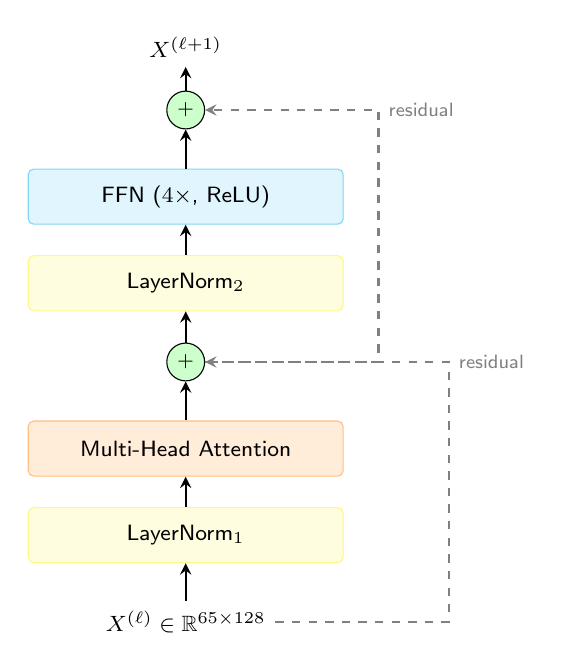
\begin{tikzpicture}[
    block/.style={draw, rounded corners=2pt, minimum width=4.0cm,
                  minimum height=0.7cm, align=center,
                  font=\footnotesize\sffamily, inner sep=4pt},
    op/.style={draw, circle, inner sep=2pt,
               font=\scriptsize\bfseries},
    arw/.style={->, >=stealth, thick},
    skip/.style={->, >=stealth, thick, dashed, gray},
]
% --- Input ---
\node[font=\footnotesize\sffamily] (input) at (0, -0.3)
    {$X^{(\ell)} \in \mathbb{R}^{65 \times 128}$};

% --- LN1 ---
\node[block, fill=yellow!12, draw=yellow!50] (ln1) at (0, 0.8)
    {LayerNorm$_1$};

% --- MHA ---
\node[block, fill=orange!15, draw=orange!50] (mha) at (0, 1.9)
    {Multi-Head Attention};

% --- Add 1 ---
\node[op, fill=green!20] (add1) at (0, 3.0) {$+$};

% --- LN2 ---
\node[block, fill=yellow!12, draw=yellow!50] (ln2) at (0, 4.0)
    {LayerNorm$_2$};

% --- FFN ---
\node[block, fill=cyan!12, draw=cyan!50] (ffn) at (0, 5.1)
    {FFN ($4\times$, ReLU)};

% --- Add 2 ---
\node[op, fill=green!20] (add2) at (0, 6.2) {$+$};

% --- Output ---
\node[font=\footnotesize\sffamily] (output) at (0, 7.0)
    {$X^{(\ell+1)}$};

% --- Main flow ---
\draw[arw] (input) -- (ln1);
\draw[arw] (ln1) -- (mha);
\draw[arw] (mha) -- (add1);
\draw[arw] (add1) -- (ln2);
\draw[arw] (ln2) -- (ffn);
\draw[arw] (ffn) -- (add2);
\draw[arw] (add2) -- (output);

% --- Residual connections ---
\draw[skip] (input.east) -- ++(2.2, 0) |- (add1.east)
    node[pos=0.5, right, font=\scriptsize\sffamily, text=gray]
    {residual};
\draw[skip] (add1.east) -- ++(2.2, 0) |- (add2.east)
    node[pos=0.5, right, font=\scriptsize\sffamily, text=gray]
    {residual};
\end{tikzpicture}
\caption{Internal structure of a single Pre-LN Transformer block
(Architecture B). Unlike the Post-LN variant (Figure~\ref{fig:encoder_block}),
normalization is applied \textit{before} each sublayer. The input
$X^{(\ell)}$ bypasses each sublayer via dashed residual paths, which
are summed ($+$) with the sublayer output. The MHA sublayer is where
the Differential or MtG attention mechanism is applied.}
\label{fig:vit_block}
\end{figure}

\paragraph{Why two architectures?}
The hybrid CNN--Transformer (Architecture A) serves as the experimental
platform within the Synthetic Observer web application, enabling rapid
training and interactive visualization of vanilla vs.\ residual attention
dynamics. The Vision Transformer (Architecture B) is used for the
Differential and Mind the Gap experiments in Google Colab, where the
full $65 \times 65$ attention matrix provides the rich spectral
structure necessary for meaningful stable rank analysis. Both
architectures share $d = 128$ and $h = 4$ heads, ensuring that
attention-level comparisons remain valid.

Two standard image classification benchmarks are supported by the
experimental platform:

\paragraph{CIFAR-10}~(Krizhevsky, 2009) is the primary dataset used in
all experiments reported in this work. It consists of 60{,}000 color
images of size $32 \times 32 \times 3$ distributed across 10 classes
(airplane, automobile, bird, cat, deer, dog, frog, horse, ship, truck),
with 50{,}000 training and 10{,}000 test images. Preprocessing consists
of resizing to $32 \times 32$ (identity transform for CIFAR-10) and
channel-wise normalization to zero mean and unit variance:
\begin{equation}
    x_{\text{norm}} = \frac{x - 0.5}{0.5}, \quad x \in [0, 1].
    \label{eq:cifar_norm}
\end{equation}

\paragraph{MNIST}~(LeCun et al., 1998) serves as a secondary validation
dataset. It contains 70{,}000 grayscale handwritten digit images of size
$28 \times 28 \times 1$ across 10 classes (digits 0--9), with 60{,}000
training and 10{,}000 test images. When selected, the convolutional
front-end is adjusted to accept single-channel input (32 filters in
Conv1 instead of 64), and two $2 \times 2$ max-pooling operations reduce
the spatial dimensions from $28 \times 28$ to $7 \times 7$.

\begin{table}[H]
\centering
\caption{Dataset summary.}
\label{tab:datasets}
\begin{tabular}{@{}lcccc@{}}
\toprule
\textbf{Dataset} & \textbf{Image Size} & \textbf{Channels} & \textbf{Classes} & \textbf{Train / Test} \\
\midrule
CIFAR-10 & $32 \times 32$ & 3 (RGB) & 10 & 50{,}000 / 10{,}000 \\
MNIST    & $28 \times 28$ & 1 (Gray) & 10 & 60{,}000 / 10{,}000 \\
\bottomrule
\end{tabular}
\end{table}

\subsection{Model Architecture}

The experiments in this work use two distinct architectures, each sharing
the same attention hidden dimension $d = 128$ and $h = 4$ heads, but
differing in how the input image is tokenized:

\paragraph{Architecture A: Hybrid CNN--Transformer (Vanilla \& Residual).}
Used in the Synthetic Observer web application for the vanilla and
residual attention experiments. A convolutional front-end extracts
features and reduces spatial dimensions before a single-token attention
stack:
\begin{enumerate}[label=\arabic*.]
    \item \texttt{Conv2d}$(3 \to 64,\; 3\times 3,\; \text{pad}=1)$ +
          BatchNorm2d(64) + ReLU + MaxPool$(2\times 2)$
    \item \texttt{Conv2d}$(64 \to 64,\; 3\times 3,\; \text{pad}=1)$ +
          BatchNorm2d(64) + ReLU + MaxPool$(2\times 2)$
    \item Flatten $\to$ FC$(4096 \to 128)$ $\to$ unsqueeze to
          $B \times 1 \times 128$
\end{enumerate}
Classification head: FC$(128 \to 10)$.

\paragraph{Architecture B: Vision Transformer (Differential \& Mind the Gap).}
Used in the standalone Colab experiments for the differential and
Mind the Gap attention variants. This is a proper ViT with patch
embedding:
\begin{enumerate}[label=\arabic*.]
    \item \textbf{Patch embedding:}
          \texttt{Conv2d}$(3 \to 128,\; 4\times 4,\;
          \text{stride}=4)$ splits a $32 \times 32$ image into
          $(32/4)^2 = 64$ non-overlapping patches, each projected to
          $d = 128$.
    \item \textbf{CLS token:} A learnable $[\text{CLS}]$ token
          ($\in \mathbb{R}^{1 \times 128}$) is prepended, yielding
          $n = 65$ tokens.
    \item \textbf{Positional encoding:} Learnable positional embeddings
          $\in \mathbb{R}^{65 \times 128}$ are added.
    \item \textbf{Attention stack:} $L = 6$ Pre-LN Transformer blocks.
    \item \textbf{Classification:} Final LayerNorm $\to$ extract
          $[\text{CLS}]$ token $\to$ FC$(128 \to 10)$.
\end{enumerate}

This dual-architecture approach allows the vanilla and residual
experiments to run rapidly via the web app (single-token attention),
while the differential and MtG experiments operate on a full 65-token
sequence where the attention matrix $A \in \mathbb{R}^{65 \times 65}$
has meaningful spectral structure for stable rank analysis.

\subsubsection{Vanilla Attention Block}

The vanilla attention block implements scaled dot-product self-attention
followed by a single-layer FFN, with \textit{no} residual connections
and \textit{no} layer normalization:
\begin{align}
    H &= \text{MHA}(X, X, X), \label{eq:vanilla_mha} \\
    Y &= W_{\text{ff}}\, H + b_{\text{ff}}, \label{eq:vanilla_ff}
\end{align}
where $\text{MHA}$ uses $h = 4$ heads with $d_k = d/h = 32$, and
$W_{\text{ff}} \in \mathbb{R}^{128 \times 128}$.

\paragraph{Design rationale.}
This block serves as the \textbf{negative control}. By stripping away
all stabilization mechanisms, we expose the raw spectral dynamics of the
attention matrix. The hypothesis is that without the identity bypass
(residual) and scale normalization (LayerNorm), the attention matrix's
spectral gap will cause progressive rank collapse across layers,
manifesting as rapidly decaying stable rank and degraded training
performance.

\paragraph{Parameter count.}
For $d = 128$ and $h = 4$: MHA contributes $4 \times (128 \times 32)
\times 3 + 128 \times 128 = 65{,}536$ parameters (Q, K, V projections
plus output projection); FFN contributes $128 \times 128 + 128 =
16{,}512$ parameters. Total per block: ${\sim}82$K.

\subsubsection{Residual Attention Block}

The residual attention block implements the standard Transformer encoder
block with Post-LN residual connections and an expanded two-layer FFN
with GELU activation:
\begin{align}
    H &= \text{LayerNorm}\!\left(X + \text{MHA}(X, X, X)\right),
    \label{eq:res_mha} \\
    Y &= \text{LayerNorm}\!\left(H + W_2\,
        \text{GELU}(W_1\, H + b_1) + b_2\right),
    \label{eq:res_ff}
\end{align}
where $W_1 \in \mathbb{R}^{128 \times 512}$ and
$W_2 \in \mathbb{R}^{512 \times 128}$ implement the $4\times$ expansion
FFN, and both LayerNorm layers have learnable $\gamma, \beta \in
\mathbb{R}^{128}$.

\paragraph{Design rationale.}
This block serves as the \textbf{positive control}---it is the closest
to the standard Transformer encoder block. The residual connection
preserves a signal floor (Section~4.4), and the expanded FFN with GELU
provides greater per-token representational capacity than the single
linear layer in the vanilla block.

\paragraph{Parameter count.}
MHA: ${\sim}66$K (same as vanilla). FFN: $128 \times 512 + 512 +
512 \times 128 + 128 = 131{,}712$. Two LayerNorm: $2 \times 256 = 512$.
Total per block: ${\sim}198$K.

\subsubsection{Differential Attention Block}

The differential attention block (\texttt{DiffHead}) implements the
mechanism described in Section~4.6 within a \textbf{Pre-LN residual}
Transformer block. Each head maintains dual query and key projections
with a shared value projection:
\begin{align}
    A_1 &= \text{softmax}\!\left(\frac{(XW_1^Q)(XW_1^K)^\top}
           {\sqrt{C}}\right), \quad
    A_2 = \text{softmax}\!\left(\frac{(XW_2^Q)(XW_2^K)^\top}
           {\sqrt{C}}\right), \label{eq:impl_diff_maps} \\
    \text{head}_i &= (A_1 - \alpha\, A_2)\, (X W^V),
    \label{eq:impl_diff_out}
\end{align}
where $\alpha$ is a \textbf{learnable scalar} initialized to
$\alpha_{\text{init}} = 0.5$ (\texttt{nn.Parameter(torch.tensor(0.5))}).
The $h = 4$ head outputs are concatenated and projected through
$W^O \in \mathbb{R}^{128 \times 128}$.

The block is wrapped in a \textbf{Pre-LN residual} structure:
\begin{align}
    H &= X + \text{MHA}_{\text{diff}}(\text{LN}_1(X)),
    \label{eq:impl_diff_preln} \\
    Y &= H + \text{FFN}(\text{LN}_2(H)),
    \label{eq:impl_diff_ffn}
\end{align}
where the FFN uses $4\times$ expansion with ReLU:
$\text{FFN}(z) = W_2\, \text{ReLU}(W_1 z)$, with
$W_1 \in \mathbb{R}^{128 \times 512}$ and
$W_2 \in \mathbb{R}^{512 \times 128}$.

\paragraph{Design rationale.}
Unlike the vanilla block, the differential attention experiment retains
residual connections and layer normalization, matching the standard
Pre-LN Transformer. This deliberate choice isolates the spectral effect
of the $A_1 - \alpha A_2$ subtraction: any improvement in stable rank
over the residual baseline can be attributed to the differential
mechanism itself, not to the absence of stabilization.

\subsubsection{Mind the Gap Attention Block}

The Mind the Gap (MtG) attention block (\texttt{MTGHead}) implements a
practical approximation of the spectral gap correction described in
Section~4.7. Rather than performing an explicit SVD on the attention
matrix---which would be computationally expensive for longer
sequences---our implementation applies \textbf{pre-softmax mean centering
and variance normalization} to the raw attention logits, which
achieve an equivalent effect of flattening the singular value spectrum:
\begin{align}
    S &= \frac{QK^\top}{\sqrt{C}},
    \label{eq:impl_mtg_raw} \\
    \bar{S} &= S - \underbrace{\frac{1}{T}\sum_{j=1}^{T}
    S_{\cdot,j}}_{\text{row mean}},
    \label{eq:impl_mtg_center} \\
    \hat{S} &= \frac{\bar{S}}{\sqrt{\text{Var}(\bar{S}) + \epsilon}},
    \quad \epsilon = 10^{-5},
    \label{eq:impl_mtg_norm} \\
    A &= \text{softmax}(\hat{S}),
    \label{eq:impl_mtg_softmax} \\
    Y &= A\, V.
    \label{eq:impl_mtg_out}
\end{align}

\paragraph{Why centering approximates spectral gap correction.}
The mean centering step (Eq.~\ref{eq:impl_mtg_center}) removes the
DC component of each row of the logit matrix. Since the spectral gap
in the softmax attention matrix arises primarily from the uniform
component of the logits (which contributes to $\sigma_1 = 1$),
subtracting the row mean suppresses this uniform bias \textit{before}
the softmax is applied. The subsequent variance normalization
(Eq.~\ref{eq:impl_mtg_norm}) ensures that the logit magnitudes are
controlled, preventing the softmax from saturating into a near-one-hot
distribution. Together, these two operations produce an attention matrix
with a significantly reduced spectral gap and correspondingly higher
stable rank---without the $\mathcal{O}(n^3)$ cost of an explicit SVD.

The block is wrapped in a \textbf{Pre-LN residual} structure identical
to the differential block (Eqs.~\ref{eq:impl_diff_preln}--\ref{eq:impl_diff_ffn}).

\paragraph{Design rationale.}
This block tests whether a lightweight, differentiable approximation to
the spectral gap correction can achieve the same stabilizing effect as
the full SVD-based approach. By normalizing logits rather than clamping
singular values, the MtG block remains fully compatible with standard
autograd and adds negligible computational overhead.

\paragraph{Summary of attention variants.}
Table~\ref{tab:attention_variants} compares the four implementations.

\begin{table}[H]
\centering
\caption{Comparison of the four attention block variants.}
\label{tab:attention_variants}
\begin{tabular}{@{}lccccc@{}}
\toprule
\textbf{Variant} & \textbf{Arch.} & \textbf{Residual} & \textbf{LN}
    & \textbf{FFN} & \textbf{Special Mechanism} \\
\midrule
Vanilla      & A (CNN) & $\times$ & $\times$
    & $1\times$ & None \\
Residual     & A (CNN) & \checkmark & \checkmark
    & $4\times$ GELU & None \\
Differential & B (ViT) & \checkmark & \checkmark
    & $4\times$ ReLU & $A_1 - \alpha A_2$ \\
Mind the Gap & B (ViT) & \checkmark & \checkmark
    & $4\times$ ReLU & Logit centering + norm \\
\bottomrule
\end{tabular}
\end{table}

\subsection{Training Pipeline}

This subsection traces the journey of a single $32 \times 32$ CIFAR-10
image through both architectures, tracking tensor dimensions at every
stage. Understanding this data flow is essential for interpreting the
stable rank measurements reported in Section~7.

\subsubsection{Pipeline A: Hybrid CNN--Transformer (Vanilla / Residual)}

Figure~\ref{fig:pipeline_a} illustrates the data flow.

\begin{figure}[H]
\centering
\resizebox{0.95\textwidth}{!}{%
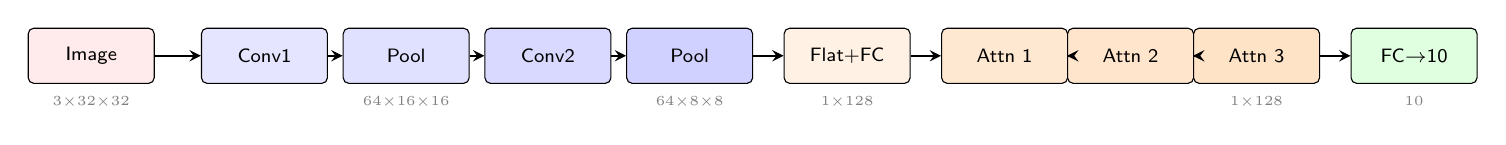
\begin{tikzpicture}[
    box/.style={draw, rounded corners=2pt, minimum height=0.7cm,
                align=center, font=\scriptsize\sffamily,
                minimum width=1.6cm, inner sep=3pt},
    arw/.style={->, >=stealth, thick},
    dm/.style={font=\tiny\sffamily, text=gray},
]
\node[box, fill=red!8] (img) at (0,0) {Image};
\node[box, fill=blue!10] (c1) at (2.2,0) {Conv1};
\node[box, fill=blue!12] (p1) at (4.0,0) {Pool};
\node[box, fill=blue!15] (c2) at (5.8,0) {Conv2};
\node[box, fill=blue!18] (p2) at (7.6,0) {Pool};
\node[box, fill=orange!10] (fl) at (9.6,0) {Flat+FC};
\node[box, fill=orange!18] (a1) at (11.6,0) {Attn~1};
\node[box, fill=orange!20] (a2) at (13.2,0) {Attn~2};
\node[box, fill=orange!22] (a3) at (14.8,0) {Attn~3};
\node[box, fill=green!12] (cl) at (16.8,0) {FC$\to$10};

\foreach \a/\b in {img/c1, c1/p1, p1/c2, c2/p2, p2/fl, fl/a1, a1/a2, a2/a3, a3/cl}
    \draw[arw] (\a) -- (\b);

\node[dm, below=1pt] at (img.south) {$3{\times}32{\times}32$};
\node[dm, below=1pt] at (p1.south) {$64{\times}16{\times}16$};
\node[dm, below=1pt] at (p2.south) {$64{\times}8{\times}8$};
\node[dm, below=1pt] at (fl.south) {$1{\times}128$};
\node[dm, below=1pt] at (a3.south) {$1{\times}128$};
\node[dm, below=1pt] at (cl.south) {$10$};
\end{tikzpicture}%
}
\caption{Pipeline A data flow (vanilla / residual attention experiments).}
\label{fig:pipeline_a}
\end{figure}

\paragraph{Step 1: Input.}
A CIFAR-10 image $x \in \mathbb{R}^{3 \times 32 \times 32}$ is
normalized to $[-1, 1]$. A minibatch of $B = 32$ images yields
$X \in \mathbb{R}^{32 \times 3 \times 32 \times 32}$.

\paragraph{Step 2--3: Convolutional blocks.}
$\text{Conv}_{3\times3}^{3 \to 64}$ + BN + ReLU + MaxPool$_{2\times2}$
$\to \mathbb{R}^{B \times 64 \times 16 \times 16}$;
then $\text{Conv}_{3\times3}^{64 \to 64}$ + BN + ReLU +
MaxPool$_{2\times2}$
$\to \mathbb{R}^{B \times 64 \times 8 \times 8}$.

\paragraph{Step 4: Flatten and project.}
Flatten $\to \mathbb{R}^{B \times 4096}$, then FC$(4096 \to 128)$
$\to \mathbb{R}^{B \times 128}$, unsqueeze $\to
\mathbb{R}^{B \times 1 \times 128}$ (single token, $n=1$).

\paragraph{Step 5: Attention stack.}
$L = 3$ attention blocks, each preserving shape
$\mathbb{R}^{B \times 1 \times 128}$. The attention matrix per head is
$A \in \mathbb{R}^{1 \times 1}$ (trivial for $n=1$).

\paragraph{Step 6: Classification.}
Squeeze $\to \mathbb{R}^{B \times 128}$, then FC$(128 \to 10)$.

\subsubsection{Pipeline B: Vision Transformer (Differential / Mind the Gap)}

Figure~\ref{fig:pipeline_b} illustrates the ViT data flow used in the
stable rank analysis experiments.

\begin{figure}[H]
\centering
\resizebox{0.95\textwidth}{!}{%
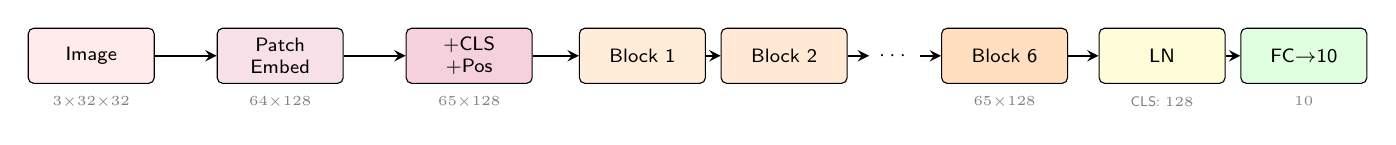
\begin{tikzpicture}[
    box/.style={draw, rounded corners=2pt, minimum height=0.7cm,
                align=center, font=\scriptsize\sffamily,
                minimum width=1.6cm, inner sep=3pt},
    arw/.style={->, >=stealth, thick},
    dm/.style={font=\tiny\sffamily, text=gray},
]
\node[box, fill=red!8] (img) at (0,0) {Image};
\node[box, fill=purple!12] (pe) at (2.4,0) {Patch\\Embed};
\node[box, fill=purple!18] (cls) at (4.8,0) {+CLS\\+Pos};
\node[box, fill=orange!15] (b1) at (7.0,0) {Block~1};
\node[box, fill=orange!17] (b2) at (8.8,0) {Block~2};
\node[font=\scriptsize\sffamily] (dots) at (10.2,0) {$\cdots$};
\node[box, fill=orange!25] (bL) at (11.6,0) {Block~6};
\node[box, fill=yellow!15] (ln) at (13.6,0) {LN};
\node[box, fill=green!12] (hd) at (15.4,0) {FC$\to$10};

\foreach \a/\b in {img/pe, pe/cls, cls/b1, b1/b2, b2/dots, dots/bL, bL/ln, ln/hd}
    \draw[arw] (\a) -- (\b);

\node[dm, below=1pt] at (img.south) {$3{\times}32{\times}32$};
\node[dm, below=1pt] at (pe.south) {$64{\times}128$};
\node[dm, below=1pt] at (cls.south) {$65{\times}128$};
\node[dm, below=1pt] at (bL.south) {$65{\times}128$};
\node[dm, below=1pt] at (ln.south) {CLS: $128$};
\node[dm, below=1pt] at (hd.south) {$10$};
\end{tikzpicture}%
}
\caption{Pipeline B data flow (differential / MtG attention experiments).
The $32 \times 32$ image is split into 64 patches of size $4 \times 4$,
each projected to $d = 128$. A CLS token is prepended, yielding
$n = 65$ tokens. The attention matrix $A \in \mathbb{R}^{65 \times 65}$
has rich spectral structure suitable for stable rank analysis.}
\label{fig:pipeline_b}
\end{figure}

\paragraph{Step 1: Patch embedding.}
\texttt{Conv2d}$(3 \to 128,\; 4 \times 4,\; \text{stride}=4)$ splits the
image into $(32/4)^2 = 64$ patches:
\begin{equation}
    X_{\text{patches}} = \text{PatchEmbed}(x)
    \in \mathbb{R}^{B \times 64 \times 128}.
    \label{eq:patch_embed}
\end{equation}

\paragraph{Step 2: CLS token and positional encoding.}
A learnable CLS token $z_{\text{cls}} \in \mathbb{R}^{1 \times 128}$
is prepended, and learnable positional embeddings are added:
\begin{equation}
    X^{(0)} = [z_{\text{cls}}; X_{\text{patches}}]
    + E_{\text{pos}} \in \mathbb{R}^{B \times 65 \times 128},
    \label{eq:cls_pos}
\end{equation}
where $E_{\text{pos}} \in \mathbb{R}^{65 \times 128}$.

\paragraph{Step 3: Transformer blocks.}
$L = 6$ Pre-LN blocks, each with the appropriate attention mechanism
(Differential or MtG). Each block preserves shape
$\mathbb{R}^{B \times 65 \times 128}$ and produces attention matrices
$A^{(\ell)}_h \in \mathbb{R}^{65 \times 65}$ per head.

\paragraph{Step 4: Classification.}
Final LayerNorm, extract CLS token ($X^{(L)}_{\cdot,0,\cdot}
\in \mathbb{R}^{B \times 128}$), and project:
$\hat{y} = W_{\text{head}}\, x_{\text{cls}} \in
\mathbb{R}^{B \times 10}$.

\subsubsection{Stable Rank Computation}

The stable rank is computed every 50 training steps on the attention
matrices from the first 2 heads to reduce overhead:
\begin{equation}
    r(A) = \frac{\|A\|_F^2}{\|A\|_2^2 + \epsilon},
    \quad \epsilon = 10^{-8},
    \label{eq:sr_impl}
\end{equation}
where $A \in \mathbb{R}^{65 \times 65}$ and $\|A\|_2 = \sigma_1$
is obtained via \texttt{torch.linalg.svdvals}. The per-layer stable
ranks are averaged across the batch and the two sampled heads.

\subsubsection{Loss and Optimization}

Both pipelines use \textbf{cross-entropy loss}:
\begin{equation}
    \mathcal{L} = -\frac{1}{B}\sum_{i=1}^{B}
    \log\frac{\exp(\hat{y}_{i,c_i})}{\sum_{j=1}^{C}\exp(\hat{y}_{i,j})}.
    \label{eq:cross_entropy}
\end{equation}

Optimization uses \textbf{AdamW}. Hyperparameters differ slightly
between pipelines:

\begin{table}[H]
\centering
\caption{Training hyperparameters for each pipeline.}
\label{tab:hyperparams}
\begin{tabular}{@{}lcc@{}}
\toprule
\textbf{Hyperparameter} & \textbf{Pipeline A} & \textbf{Pipeline B} \\
\midrule
Batch size $B$       & 32                 & 128 \\
Learning rate        & $1 \times 10^{-3}$ & $3 \times 10^{-4}$ \\
LR schedule          & Cosine annealing   & None (constant) \\
Weight decay          & 0                  & 0 \\
Attention layers $L$ & 3                  & 6 \\
Heads $h$            & 4                  & 4 \\
Hidden dim $d$       & 128                & 128 \\
\bottomrule
\end{tabular}
\end{table}

\subsubsection{Dimension Summary}

Table~\ref{tab:dimensions} provides a complete reference of tensor
dimensions through both pipelines.

\begin{table}[H]
\centering
\caption{Tensor dimensions for Pipeline A (CNN) and Pipeline B (ViT).
$B$ denotes batch size.}
\label{tab:dimensions}
\begin{tabular}{@{}llcc@{}}
\toprule
\textbf{Stage} & \textbf{Operation}
    & \textbf{Pipeline A} & \textbf{Pipeline B} \\
\midrule
Input    & ---
    & $B{\times}3{\times}32{\times}32$ & $B{\times}3{\times}32{\times}32$ \\
Tokenize & Conv / Patch
    & $B{\times}64{\times}8{\times}8$ & $B{\times}64{\times}128$ \\
Project  & FC / +CLS+Pos
    & $B{\times}1{\times}128$ & $B{\times}65{\times}128$ \\
Attn.    & $\times L$ blocks
    & $B{\times}1{\times}128$ & $B{\times}65{\times}128$ \\
Attn.~matrix & per head
    & $1{\times}1$ & $65{\times}65$ \\
Classify & FC
    & $B{\times}10$ & $B{\times}10$ \\
\bottomrule
\end{tabular}
\end{table}

\subsection{Tools, Libraries, and Frameworks}

Table~\ref{tab:tools} lists the principal software components used in
this project.

\begin{table}[H]
\centering
\caption{Software stack.}
\label{tab:tools}
\begin{tabular}{@{}lll@{}}
\toprule
\textbf{Component} & \textbf{Tool / Library} & \textbf{Role} \\
\midrule
Deep Learning   & PyTorch 2.x       & Model definition, training, autograd \\
Data Loading    & torchvision       & CIFAR-10 / MNIST datasets, transforms \\
Backend API     & FastAPI           & REST API for training orchestration \\
Database        & SQLAlchemy + SQLite & Training session persistence \\
Frontend        & React 18 + Vite   & Interactive dashboard UI \\
Styling         & Tailwind CSS 3.4  & Responsive layout and styling \\
Animations      & Framer Motion     & Architecture visualization animations \\
Icons           & Lucide React      & UI iconography \\
HTTP Client     & Axios             & Frontend--backend communication \\
Containerization & Docker Compose   & Reproducible deployment \\
Notebook        & Google Colab      & Stable rank analysis experiments \\
Typesetting     & \LaTeX{} + TikZ   & Report preparation and diagrams \\
\bottomrule
\end{tabular}
\end{table}

\subsection{Web Application --- Synthetic Observer}

The \textbf{Synthetic Observer} is a full-stack web application designed
to provide real-time, interactive visualization of Transformer training
dynamics. It serves as both an experimental workbench and a pedagogical
tool.

\paragraph{Architecture.}
The application follows a client--server architecture:
\begin{itemize}[leftmargin=1.5em]
    \item \textbf{Backend} (FastAPI, port 8000): Manages training
          sessions, dispatches model training as background tasks,
          caches weight snapshots per epoch, and exposes REST endpoints
          for training control (\texttt{/train}), weight retrieval
          (\texttt{/weights/\{session\_id\}}), and session management.
    \item \textbf{Frontend} (React + Vite, port 3000): Provides a
          dashboard with configurable hyperparameters (attention type,
          number of layers, heads, epochs, learning rate, dataset),
          real-time training metric charts (loss, accuracy, learning
          rate decay, validation error), and an animated architecture
          diagram that visually represents the attention blocks and
          heads.
    \item \textbf{Colab integration}: A Google Colab notebook for
          stable rank analysis of the differential attention matrix is
          embedded into the dashboard via a server-side proxy endpoint
          (\texttt{/api/colab/notebook}), allowing users to view
          experimental results without leaving the application.
\end{itemize}

\paragraph{Key features.}
\begin{enumerate}[label=(\roman*)]
    \item \textbf{Side-by-side comparison}: Users can train vanilla and
          residual attention models under identical hyperparameters and
          observe diverging loss curves and accuracy in real time.
    \item \textbf{Architecture visualization}: An animated diagram
          (Framer Motion) displays the convolutional front-end,
          attention layers, and classification head, with visual
          indicators showing the flow of data through each component.
    \item \textbf{Experiment history}: All training sessions are
          persisted in a SQLite database, enabling retrospective
          analysis and comparison across runs.
    \item \textbf{Docker deployment}: The entire stack is containerized
          via Docker Compose, ensuring identical execution environments
          across machines.
\end{enumerate}

% -----------------------------------------------------------------------------
% 6. EXPERIMENTS
% -----------------------------------------------------------------------------
\section{Experiments}

\subsection{Experimental Setup}

\subsection{Experiment 1 --- Baseline}

\subsection{Experiment 2 --- Learning Rate and Data Augmentation}

\subsection{Experiment 3 --- Increased Depth with Regularization}

\subsection{Experiment 4 --- Optimal Configuration}

\subsection{Experiment 5 --- Stable Rank Analysis on Differential Attention Matrix}

% -----------------------------------------------------------------------------
% 7. RESULTS & INTERPRETATION
% -----------------------------------------------------------------------------
\section{Results and Interpretation}

\subsection{Comparative Performance Table}

\subsection{Training Dynamics Analysis}

\subsection{Stable Rank Analysis}

\subsection{Rank Collapse Observations}

\subsection{Discussion}

% -----------------------------------------------------------------------------
% 8. CONCLUSION
% -----------------------------------------------------------------------------
\section{Conclusion}

% -----------------------------------------------------------------------------
% 9. FUTURE WORK
% -----------------------------------------------------------------------------
\section{Future Work}

% -----------------------------------------------------------------------------
% REFERENCES
% -----------------------------------------------------------------------------
\newpage
\begin{thebibliography}{99}

\bibitem{vaswani2017}
A.~Vaswani, N.~Shazeer, N.~Parmar, J.~Uszkoreit, L.~Jones, A.~N.~Gomez,
\L.~Kaiser, and I.~Polosukhin,
``Attention is all you need,''
\textit{Advances in Neural Information Processing Systems}, vol.~30, 2017.

\bibitem{diff_transformer}
T.~Ye, L.~Li, et al.,
``Differential Transformer,''
\textit{arXiv preprint arXiv:2410.05258}, 2024.

\bibitem{mind_the_gap}
N.~Noci, S.~Anagnostidis, L.~Biggio, A.~Orvieto, S.~P.~Singh, and A.~Lucchi,
``Mind the gap: A spectral analysis of rank collapse and signal propagation in Transformers,''
\textit{Advances in Neural Information Processing Systems}, 2024.

\bibitem{he2016residual}
K.~He, X.~Zhang, S.~Ren, and J.~Sun,
``Deep residual learning for image recognition,''
\textit{Proc. IEEE CVPR}, pp.~770--778, 2016.

\bibitem{ba2016layernorm}
J.~L.~Ba, J.~R.~Kiros, and G.~E.~Hinton,
``Layer normalization,''
\textit{arXiv preprint arXiv:1607.06450}, 2016.

\end{thebibliography}

% -----------------------------------------------------------------------------
% APPENDIX
% -----------------------------------------------------------------------------
\newpage
\appendix

\section{Code Repository Structure}

\section{API Documentation}

\section{Web Application Screenshots}

\section{Google Colab Notebook}

\end{document}
